%"思考Python:像计算机科学家一样思考"LaTex源码
%Copyright (c) 2008 Allen B. Downey.
%中文翻译:2010 Walter Lewis (刘宇辉).

% Permission is granted to copy, distribute and/or modify this
% document under the terms of the GNU Free Documentation License,
% Version 1.1  or any later version published by the Free Software
% Foundation; with no Invariant Sections, no Front-Cover Texts,
% and no Back-Cover Texts.

% This distribution includes a file named fdl.tex that contains the text
% of the GNU Free Documentation License.  If it is missing, you can obtain
% it from www.gnu.org or by writing to the Free Software Foundation,
% Inc., 59 Temple Place - Suite 330, Boston, MA 02111-1307, USA.
%

\documentclass[10pt]{book}
\usepackage[width=5.5in,height=8.5in,hmarginratio=3:2,vmarginratio=1:1]{geometry} %指定了{h,v}marginratio,width和height被忽略了,可以不用指定(参考geometry.pdf, $texdoc geometry.pdf)。

%下面的这些包,你可能需要安装texlive-latex-extra(in Debian/Ubuntu)
\usepackage{pslatex}  %
\usepackage{url}
\usepackage{fancyhdr}
\usepackage{graphicx}
\usepackage{amsmath,amsthm,amssymb}
\usepackage{exercise}
\usepackage{makeidx}
\usepackage{setspace}
\usepackage{hevea}
\usepackage{upquote}
%这些是对中文的支持
\usepackage{xeCJK}
\usepackage{fontspec}
\setCJKmainfont{FangSong_GB2312:style=Regular}
\setmainfont{FangSong_GB2312:style=Regular}
\XeTeXlinebreaklocale "zh"
\XeTeXlinebreakskip=0pt plus 1pt minus 0.1pt

\title{思考Python}
\newcommand{\thetitle}{思考Python:像计算机科学家一样思考}
\newcommand{\theversion}{1.1.22}

%以下的这些风格被转换成html的css
\newstyle{a:link}{color:black;}
\newstyle{p+p}{margin-top:lem;margin-bottom:lem}
\newstyle{img}{border:opx}

%改变箭头(方向)
\setlinkstext
{\imgsrc[ALT="Previous"]{back.png}}
{\imgsrc[ALT="Previous"]{up.png}}
{\imgsrc[ALT="Previous"]{next.png}}

\makeindex

\begin{document}

\frontmatter



%LaTeXOnly

\input{latexonly}

\newtheorem{ex}{Exercise}[chapter]
\begin{latexonly}

\renewcommand{\blankpage}{\thispagestyle{empty} \quad \newpage}

%blankpage
%blankpage

%-half title----------------------------------------------
\thispagestyle{empty}
\begin{flushright}
\vspace*{2.0in}

\begin{spacing}{3}
{\huge 思考Python}\\
{\Large 像计算机科学家一样思考}
\end{spacing}

\vspace{0.25in}

Version \theversion

\vfill
\end{flushright}

%---------------------------
\blankpage
\blankpage

%---title page---------
\pagebreak
\thispagestyle{empty}

\begin{flushright}
\vspace*{2.0in}

\begin{spacing}{3}
{\huge 思考Python}\\
{\Large 像计算机科学家一样思考}
\end{spacing}

\vspace{0.25in}
Version \theversion

{\Large
	Allen Downey\\
}




\vspace{0.5in}

{\Large Green Tea Press}\\
{\small Needham, Massachusetts}

\vfill
\end{flushright}

%---copyright------------------
\pagebreak
\thispagestyle{empty}

{\small
	Copyright \copyright ~2008 Allen Downey.

Printing history:

\begin{description}

\item[2002四月:] 第一版 {\em 像计算机科学家一样思考}.
\item[2007八月:] 大幅改动,把标题改为{\em 像(Python)程序员一样思考}.
\item[2008六月:] 大幅改动,把标题改为{\em 思考Python:像计算机科学家一样思考}.
\end{description}

\vspace{0.2in}

\begin{flushleft}  %左对齐,类似的有flushright,centre
Green Tea Press \\
9 Washburn Ave\\
Needham MA 02492
\end{flushleft}


Permission is granted to copy, distribute, and/or modify this document
under the terms of the GNU Free Documentation License, Version 1.1 or
any later version published by the Free Software Foundation; with no
Invariant Sections, no Front-Cover Texts, and with no Back-Cover Texts.

The GNU Free Documentation License is available from {\tt www.gnu.org}
or by writing to the Free Software Foundation, Inc., 59 Temple Place,
Suite 330, Boston, MA 02111-1307, USA.

The original form of this book is \LaTeX\ source code.  Compiling this
\LaTeX\ source has the effect of generating a device-independent
representation of a textbook, which can be converted to other formats
and printed.

The \LaTeX\ source for this book is available from
\url{http://www.thinkpython.com}
\vspace{0.2in}
}

\end{latexonly}


%htmlonly
\begin{htmlonly}

%Title page for html version

{\Large \thetitle}
\{\Large  Allen B.Downet}
\{\Large  翻译:Walter Lewis}

Version \theversion

\setcounter{chapter}{-1}
\end{htmlonly}

\chapter{前言}

\section{本书的奇怪历史}

1999年一月份的时候,我准备用Java教一门介绍性的编程课。在那之前,我已经
教了三次,而且每次我都很失望。这门课的挂课率非常之高,尽管对那些通过的学
生来说,整体的水平也是很低的。\\

我认为问题的根源之一是教科书。教科书太厚了,掺杂着大量不必要的Java细节
内容,并且没有足够高水平的引导去指导学生如何编程。学生们深陷“陷阱门“:他们起步很轻松,逐步的学习,突然,大约在第五章的某个位置,困难出现了。学生必须快速的学习大量的新内容。结果,我不得不把剩下的学期花在挑选一些片段来教学。\\

课程开始的前两周,我决定自力更生---自己编写书。我的目标是:
\begin{itemize}

\item 尽量简短.对学生来说,阅读十页比阅读五十页要好。

\item 注意词汇量。我尽量减少使用术语,而且在使用前必须先定义。

\item 逐步学习。为了避免陷阱门,我把最难的部分分解成一系列的小步骤。

\item 把重心放在编程,而不是编程语言。我采用最少的有用的Java语言的语法,
忽略其他的。
\end{itemize}

我需要一个书名,所以我就临时地把它叫做《像计算机科学家一样思考》\\

第一版很粗糙,但是很成功。学生们很乐意看它,并且能很好理解我在课堂上讲的难点,趣点和让他们实践的内容(这个最重要).\\

我用GNU自由文档许可证发布了这本书,读者们可以自由的复制,修改,发布这本书。 \\

\index{GNU Free Documentation License}
\index{Free Documentation License,GNU}

 接下来发生的事儿极其的有趣。Jeff Elkner,居住在弗尼亚的高中老师,改变了我的书,把它翻译成了Python。他给我寄了份他翻译的副本,于是乎我就有了一段不寻常的学习Python的经历--通过阅读我自己的书。\\

 Jeff和我随后修订了这本书,加入了Chris Meyers提供的一个案例学习。在2001年,我们共同发布了《像计算机科学家一样思考:Python编程》,当然同样是用GNU自由文档许可证。通过Gree Tea Press,我出版了这本书,并且开始在亚马逊和大学书店卖纸质书。Gree Tea Press出版的书可以从这儿获得\url{greenteapress.com}\\

 2003年,我开始在Olin College教书。第一次,我开始教Python。和教授Java的情况相反,学生们不再陷入泥潭,学到了更多,参与了很多有趣的项目,越学越带劲。\\

 在过去的五年里,我一直继续完善这本书,改正错误,提过某些例子的质量,加入一些其他的材料,特别是练习。在2008年,我开始重写这本书---同时,剑桥大学出版社的编辑联系到了我,他想出版本书的下一板。美妙的时刻!\\

 结构就出现了现在的这本书,不过有了一个简洁的名字《思考Python》。变化有:
 \begin{itemize}

 \item 在每一章末尾加了点调试的部分。这些部分提供了发现和避免bug的通用技巧,也对Python的陷阱提出了警告。

 \item 删除了最后几章关于列表和树实现的内容。虽然,我万分不舍,但是考虑到和本书余下的部分不协调,只能忍痛割爱。

 \item 增加了一些案例学习---提供了练习,答案和相关讨论的大例子。一些东西是基于Swampy,这是我为了教学而设计的Python程序。
 Swampy,代码实例和部分答案可以从这儿获得\url{thinkpython.com}.

 \item 扩展了关于程序构建计划和基本的设计模式的讨论。

 \item Python运用的更加地道。虽然这本书仍然是讨论编程的,而不是Python本身,但是现在我不得不承认这本书深受Python浸染。
 
 \end{itemize}

  我希望读者们可以享受这本书,也希望帮助你学习程序设计和像计算机科学家一样思考,哪怕是一丁丁点儿。\\

Allen B. Downey\\
Needham MA\\

Allen Downey 是Olin College 大学计算机科学与技术系的副教授。



\section*{声明}

首先,也是最重要的,我要感谢Jeff Elkner,是他把我的Java书翻译成了Python,也由此开启了这项“工程“,也把我领进了我最爱的编程语言大门。\\

我也要感谢Chris Meyers,他贡献了《像计算机科学家一样思考》的部分内容。\\

感谢FSF制定的GNU自由文档许可证,使我和Jeff 和Chris 的合作成为可能。\\

\index{GNU Free Documentation License}
\index{Free Documentation License,GNU}

我也要感谢所以使用以前版本的学生和所有的贡献者,他们提供了宝贵的更正和建议2。\\

感谢我的妻子,Lisa为她在这本书上所花费的努力,还有Gree Tea Press,和其他的一切。

\section*{贡献者名单}

\index{贡献者}

More than 100 sharp-eyed and thoughtful readers have sent in
suggestions and corrections over the past few years.  Their
contributions, and enthusiasm for this project, have been a
huge help.

If you have a suggestion or correction, please send email to 
{\tt feedback@thinkpython.com}.  If I make a change based on your
feedback, I will add you to the contributor list
(unless you ask to be omitted).

If you include at least part of the sentence the
error appears in, that makes it easy for me to search.  Page and
section numbers are fine, too, but not quite as easy to work with.
Thanks!

\small

\begin{itemize}

\item Lloyd Hugh Allen sent in a correction to Section 8.4.

\item Yvon Boulianne sent in a correction of a semantic error in
Chapter 5.

\item Fred Bremmer submitted a correction in Section 2.1.

\item Jonah Cohen wrote the Perl scripts to convert the
LaTeX source for this book into beautiful HTML.

\item Michael Conlon sent in a grammar correction in Chapter 2
and an improvement in style in Chapter 1, and he initiated discussion
on the technical aspects of interpreters.

\item Benoit Girard sent in a
correction to a humorous mistake in Section 5.6.

\item Courtney Gleason and Katherine Smith wrote {\tt horsebet.py},
which was used as a case study in an earlier version of the book.  Their
program can now be found on the website.

\item Lee Harr submitted more corrections than we have room to list
here, and indeed he should be listed as one of the principal editors
of the text.

\item James Kaylin is a student using the text. He has submitted
numerous corrections.

\item David Kershaw fixed the broken {\tt catTwice} function in Section
3.10.

\item Eddie Lam has sent in numerous corrections to Chapters 
1, 2, and 3.
He also fixed the Makefile so that it creates an index the first time it is
run and helped us set up a versioning scheme.  

\item Man-Yong Lee sent in a correction to the example code in
Section 2.4.  

\item David Mayo pointed out that the word ``unconsciously"
in Chapter 1 needed
to be changed to ``subconsciously".

\item Chris McAloon sent in several corrections to Sections 3.9 and
3.10.

\item Matthew J. Moelter has been a long-time contributor who sent
in numerous corrections and suggestions to the book.  

\item Simon Dicon Montford reported a missing function definition and
several typos in Chapter 3.  He also found errors in the {\tt increment}
function in Chapter 13.

\item John Ouzts corrected the definition of ``return value"
in Chapter 3.

\item Kevin Parks sent in valuable comments and suggestions as to how
to improve the distribution of the book.

\item David Pool sent in a typo in the glossary of Chapter 1, as well
as kind words of encouragement.

\item Michael Schmitt sent in a correction to the chapter on files
and exceptions.

\item Robin Shaw pointed out an error in Section 13.1, where the
printTime function was used in an example without being defined.

\item Paul Sleigh found an error in Chapter 7 and a bug in Jonah Cohen's
Perl script that generates HTML from LaTeX.

\item Craig T. Snydal is testing the text in a course at Drew
University.  He has contributed several valuable suggestions and corrections.

\item Ian Thomas and his students are using the text in a programming
course.  They are the first ones to test the chapters in the latter half
of the book, and they have made numerous corrections and suggestions.

\item Keith Verheyden sent in a correction in Chapter 3.

\item Peter Winstanley let us know about a longstanding error in
our Latin in Chapter 3.

\item Chris Wrobel made corrections to the code in the chapter on
file I/O and exceptions. 

\item Moshe Zadka has made invaluable contributions to this project.
In addition to writing the first draft of the chapter on Dictionaries, he
provided continual guidance in the early stages of the book.

\item Christoph Zwerschke sent several corrections and
pedagogic suggestions, and explained the difference between {\em gleich}
and {\em selbe}.

\item James Mayer sent us a whole slew of spelling and
typographical errors, including two in the contributor list.

\item Hayden McAfee caught a potentially confusing inconsistency
between two examples.

\item Angel Arnal is part of an international team of translators
working on the Spanish version of the text.  He has also found several
errors in the English version.

\item Tauhidul Hoque and Lex Berezhny created the illustrations
in Chapter 1 and improved many of the other illustrations.

\item Dr. Michele Alzetta caught an error in Chapter 8 and sent
some interesting pedagogic comments and suggestions about Fibonacci
and Old Maid.

\item Andy Mitchell caught a typo in Chapter 1 and a broken example
in Chapter 2.

\item Kalin Harvey suggested a clarification in Chapter 7 and
caught some typos.

\item Christopher P. Smith caught several typos and helped us
update the book for Python 2.2.

\item David Hutchins caught a typo in the Foreword.

\item Gregor Lingl is teaching Python at a high school in Vienna,
Austria.  He is working on a German translation of the book,
and he caught a couple of bad errors in Chapter 5.

\item Julie Peters caught a typo in the Preface.

\item Florin Oprina sent in an improvement in {\tt makeTime},
a correction in {\tt printTime}, and a nice typo.

\item D.~J.~Webre suggested a clarification in Chapter 3.

\item Ken found a fistful of errors in Chapters 8, 9 and 11.

\item Ivo Wever caught a typo in Chapter 5 and suggested a clarification
in Chapter 3.

\item Curtis Yanko suggested a clarification in Chapter 2.

\item Ben Logan sent in a number of typos and problems with translating
the book into HTML.

\item Jason Armstrong saw the missing word in Chapter 2.

\item Louis Cordier noticed a spot in Chapter 16 where the code
didn't match the text.

\item Brian Cain suggested several clarifications in Chapters 2 and 3.

\item Rob Black sent in a passel of corrections, including some
changes for Python 2.2.

\item Jean-Philippe Rey at Ecole Centrale
Paris sent a number of patches, including some updates for Python 2.2
and other thoughtful improvements.

\item Jason Mader at George Washington University made a number
of useful suggestions and corrections.

\item Jan Gundtofte-Bruun reminded us that ``a error'' is an error.

\item Abel David and Alexis Dinno reminded us that the plural of
``matrix'' is ``matrices'', not ``matrixes''.  This error was in the
book for years, but two readers with the same initials reported it on
the same day.  Weird.

\item Charles Thayer encouraged us to get rid of the semi-colons
we had put at the ends of some statements and to clean up our
use of ``argument'' and ``parameter''.

\item Roger Sperberg pointed out a twisted piece of logic in Chapter 3.

\item Sam Bull pointed out a confusing paragraph in Chapter 2.

\item Andrew Cheung pointed out two instances of ``use before def.''

\item C. Corey Capel spotted the missing word in the Third Theorem
of Debugging and a typo in Chapter 4.

\item Alessandra helped clear up some Turtle confusion.

\item Wim Champagne found a brain-o in a dictionary example.

\item Douglas Wright pointed out a problem with floor division in
{\tt arc}.

\item Jared Spindor found some jetsam at the end of a sentence.

\item Lin Peiheng sent a number of very helpful suggestions.

\item Ray Hagtvedt sent in two errors and a not-quite-error.

\item Torsten H\"{u}bsch pointed out an inconsistency in Swampy.

\item Inga Petuhhov corrected an example in Chapter 14.

\item Arne Babenhauserheide sent several helpful corrections.

\item Mark E. Casida is is good at spotting repeated words.

\item Scott Tyler filled in a that was missing.  And then sent in
a heap of corrections.

\item Gordon Shephard sent in several corrections, all in separate
emails.

\item Andrew Turner {\tt spot}ted an error in Chapter 8.

\item Adam Hobart fixed a problem with floor division in {\tt arc}.

\item Daryl Hammond and Sarah Zimmerman pointed out that I served
up {\tt math.pi} too early.  And Zim spotted a typo.

\item George Sass found a bug in a Debugging section.

\item Brian Bingham suggested Exercise~\ref{exrotatepairs}.

\item Leah Engelbert-Fenton pointed out that I used {\tt tuple}
as a variable name, contrary to my own advice.  And then found
a bunch of typos and a ``use before def.''

\item Joe Funke spotted a typo.

\item Chao-chao Chen found an inconsistency in the Fibonacci example.

\item Jeff Paine knows the difference between space and spam.

\item Lubos Pintes sent in a typo.

\item Gregg Lind and Abigail Heithoff suggested Exercise~\ref{checksum}.

\item Max Hailperin has sent in a number of corrections and
  suggestions.  Max is one of the authors of the extraordinary {\em
    Concrete Abstractions}, which you might want to read when you are
  done with this book.

\item Chotipat Pornavalai found an error in an error message.

\item Stanislaw Antol sent a list of very helpful suggestions.

\item Eric Pashman sent a number of corrections for Chapters 4--11.

\item Miguel Azevedo found some typos.

\item Jianhua Liu sent in a long list of corrections.

\item Nick King found a missing word.

\item Martin Zuther sent a long list of suggestions.

\item Adam Zimmerman found an inconsistency in my instance
of an ``instance'' and several other errors.

\item Ratnakar Tiwari suggested a footnote explaining degenerate
triangles.

\item Anurag Goel suggested another solution for \verb"is_abecedarian"
and sent some additional corrections.  And he knows how to
spell Jane Austen.

\item Kelli Kratzer spotted one of the typos.

\item Mark Griffiths pointed out a confusing example in Chapter 3.

\item Roydan Ongie found an error in my Newton's method.

\item Patryk Wolowiec helped me with a problem in the HTML version.

\item Mark Chonofsky told me about a new keyword in Python 3.0.

\item Russell Coleman helped me with my geometry.

\item Wei Huang spotted several typographical errors.

\item Karen Barber spotted the the oldest typo in the book.

\item Nam Nguyen found a typo and pointed out that I used the Decorator
pattern but didn't mention it by name.

\item St\'{e}phane Morin sent in several corrections and suggestions.

\item Paul Stoop corrected a typo in \verb+uses_only+.

\item Eric Bronner pointed out a confusion in the discussion of the
order of operations.

\item Alexandros Gezerlis set a new standard for the number and
quality of suggestions he submitted.  We are deeply grateful!

% ENDCONTRIB

\end{itemize}


\normalsize
\clearemptydoublepage

\begin{latexonly}

\tableofcontents

\clearemptydoublepage

\end{latexonly}


\mainmatter

\chapter{编程的方式}

这本书的的目的是教会大家如何像计算机科学家一样思考。计算机科学用严谨的语言来表明思想,尤其是计算。像工程师,他们设计,把各个组件装配成系统并且在可选方案中评估出折中方案。像科学家,他们研究复杂系统的性能,做出假定并且测试假设。


\index{解决问题}

对一个计算机科学家来说最重要的是解决问题。解决问题意味着清晰明确的阐述问题,积极思考问题答案,并且清楚正确的表达答案的能力。实践证明:学习如何编程是一种很好的机会来练习解决问题的技巧。这也是为什么把这章叫做“编程的方式“。\\

一方面,你将学习编程,一个非常有用的技巧。另一方面你将会把编程作为一种科技。随着我们的深入学习,这点会渐渐明晰。

\section{Python编程语言}
\index{编程语言}
\index{语言!编程}

我们将要学习的编程语言是Python。Python仅是高级语言中的一种,你可能
也听说过其他的高级编程语言,比如C,C++,Perl,和Java。\\

也有一些低级语言,有时也被称为机器语言或者汇编语言。一般来说,计算机
只能执行用低级语言编写的程序。所以,用高级语言编写的程序在执行前必须
做相应的处理。这会花费一定的时间,同时这也是高级语言的“缺点“。\\

\index{移植性}
\index{高级语言}
\index{低级语言}
\index{语言!高级}
\index{语言!低级}

然而,高级语言的优点也是无限的。首先,用高级语言编程是一件非常容易的。
用高级语言编程通常花费的时间比较少,同时编写的程序简短,易读,易纠错
。第二,高级语言是可移植的,这意味着他们可以不加修改(或者修改很少)地运行在不同的平台上。低级语言编写的程序只能在一个机器上运行,如果想
要运行在另外一台机器上,必须得重写。\\

基于这些优点,几乎所有的程序都是用高级语言编写的。低级语言统称仅仅用
在一些专门的应用程序中。

\index{complie}
\index{interpret}

有两种程序把高级语言“处理”成低级语言:解释器和编译器。解释器读取源程序,解释执行,也就是按照程序表达的意思"做事"。解释器一次解释一点,或者说,一次读取一行,然后执行。\\

\beforefig
\centerline{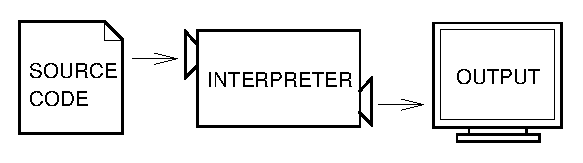
\includegraphics[height=0.77in]{figs/interpret.eps}}
\afterfig

\index{源码}
\index{目标}
\index{可执行代码}

编译器读取程序,完全转换之。在这种情况下,高级语言程序叫做源码,编译后的程序叫做目标代码或者叫可执行代码。一旦程序被编译,就可以直接执行,无须再编译。

\beforefig
\centerline{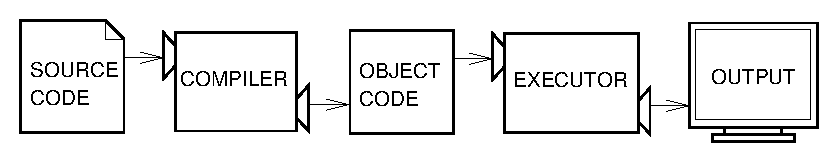
\includegraphics[height=0.77in]{figs/compile.eps}}
\afterfig

一般地,我们把python当作是解释型语言,因为用Python编写的程序是通过
解释器执行的。有两种使用解释器的方式:交互模式和脚本模式。在交互模式
下,你可以输入Python程序,然后解释器输出结果:

\index{交互模式}
\index{脚本模式}

\beforeverb
\begin{verbatim}    
>>>1 + 1
2
\end{verbatim} %直接输出以上两句,包括空白和断行
\afterverb

锯齿符,{\tt >>>},是提示符,解释器用它来表明自己已经准备好了,
如果你输入{\tt 1 + 1},解释器显示{\tt 2}。\\

\index{提示符}

另外地,我们可以把代码存储在一个文件里,使用解释器执行文件,此时这个
文件被称作脚本。习惯上,Python脚本的扩展名为{\tt .py}。

\index{脚本}

如果要执行Python脚本,我们必须提供给解释器脚本的文件名。在UNIX命令窗口,可以输入{\tt python dinsdale.py}。在其他开发环境中,会有些细节方面的差别。可以在Python官网上(\url{python.org})找到相应的指导。

\index{测试!交互模式}

在交互模式下工作很容易测试一小段代码,因为可以随时输入,并且立刻执行。但如果代码量较大,我们必须把代码存放在脚本里,这样方便我们以后修改执行。 

\section{什么是程序}

程序就是指令集合,这些指令说明了如何执行计算。计算可能是数学上的,例如解决等式组或者计算多项式的平方根。但是也可以是符号计算,比如搜索替换文件的文本或者(非常奇怪)编译一个程序。

\index{程序}

不同的语言有一些细节上的差异。但是他们有一些共有的指令:

\begin{description}

\item[输入:] 从键盘获取数据,文件,或者从其他设备。

\item[输出:] 在显示器上显示数据或者把数据输出到文件或其他设备。

\item[数学运算:] 做基本的数学操作像加法和乘法。

\item[条件执行:]检查条件,然后执行正确的语句。

\item[循环:]重复执行一些动作,通常有些变化。

\end{description}

信不信由你,就是这样。我们用过的任何一个软件,无论多么复杂,基本上都是由与这些相似的指令组成。所以,我们可以这么理解:编程就是把复杂庞大的任务分解为一系列的小任务,知道这些小任务简单到可以用这些基本的指令表示。

\index{算法}

这个有点模糊,但是当我们讲到算法的时候,我们再回过头来聊这个话题。

\section{什么是调试?}
\index{调试}
\index{臭虫}

有三种错误经常在程序中出现:语法错误,运行时错误和语义错误。为了能够快速的跟踪捕捉到他们,区分他们之间的诧异还是很有好处的。

\subsection{语法错误}
\index{语法错误}
\index{错误!语法}
\index{错误信息}

Python只能执行语法正确的程序;否则,解释器就会报错。语法指的是程序的结构和结构的规则。\index{syntax 语法}
比如,括号必须是成对出现,所以{\tt (1 + 2)}是合法的,但{\tt 8)}就是语法错误。

\index{parentheses!matching  括号!匹配}
\index{syntax 语法}
\index{cummings, e. e. 康明思}

在英语中,读者可以忍受大多数语法错误,这就是为什么我们玩味E. E康明思的诗歌,而没有提出任何错误信息的原因。Python不会这么仁慈。如果在你程序的某个地方出现了哪怕是一个语法错误,Python也会显示错误信息然后退出,你也不能再继续执行程序。在你初学编程的几周里,你很可能会花费大量的时间追踪,捕捉语法错误。一旦你有经验了,你犯的错误就更少,并且也能很快的发现他们。

\subsection{运行时错误}
\label{runtime 运行时}
\index{runtime error 运行时错误}
\index{error!runtime 错误!运行时}
\index{exception 异常}
\index{safe language 安全语言}
\index{language!safe 语言!安全}


第二中错误是运行时错误,之所以这么命名是因为从这种错误知道程序开始运行才会出现。这些错误也叫做异常,因为他们通常表明异常的事情发生了。\\

运行时错误在前几章的简短的代码中比较少见,因此你可能会有一段时间才会遇到。

\section{语义错误}
\index{semantics 语义}
\index{semantics errors 语义错误}
\index{error!semantic 错误!语义}
\index{error message 错误信息}

第三中错误是语义错误。如果有语义错误,程序会成功运行(即计算机不会产生任何的错误信息),但是它却没有做对!计算机做了另外的事。确切的说,计算机确实做了你告诉他的指令。

\subsection{试验性的调试}

你必须拥有的一条技能是调试。尽管在这个过程中,你可能很受伤,但,调试是编程中最具有挑战,最有意思,最能考验智力的一部分。\\

\index{experimental debugging 实验性的调试}
\index{debugging!experimental 调试!实验}

某种程度上,调试就像是侦探。你面对着很多线索,必须推断导致你看到的结果的过程和事件。\\

调试也像是一个科学实验。一旦你意识到错误的地方,改正她,再尝试。如果你的假想是正确的,你就可以预测出改变带来的结果,你也就离能够执行的程序更近一步了。如果你的猜想是错误的,你不得不提出一个新的。正如Sherlock Holmoes指出的,“当你移除了不可能的,留下来的无论是什么,也不论多么不可能,都是真理。(A. Conan Doyle, {\em The Sign of Four})\\

\index{Holems, Sherlock}
\index{Doyle, Arthur Conan}

对某些人来说,编程和调试是同时完成的。也就是,编程是不断调试,直到看到想要结果的过程。理念就是:你必须以一个能够工作的程序开始,然后做些小改动,随着进度不断调试他们,这样就总是有一个可工作的程序。\\

比如:Linux是一个包含成千上万行代码的操作系统,但它也是从一个Linux Torvalds用来研究Intel 80386芯片的小程序开始的。按照Larry Greenfield的说法,“Linus的早期项目就是一个在打印AAAA和BBBB之间切换的程序。“({\em The Linux Users' Guide} Beta Version 1)。

\index{Linux}

接下来的章节将介绍更多的调试建议还有其他的编程经验。

\section{正式语言和自然语言}
\index{formal language 正式语言}
\index{natural language 自然语言}
\index{language!formal 语言!正式}
\index{language!natural 语言!自然}

自然语言是人们日常说的语言,比如英语,西班牙语和法语。他们不是人民设计的(尽管人们努力的强加一些规则);他们是自然发展的。\\

正式语言是人们为了特别的应用而设计的语言。比如,数学家使用的符号就是一门正式语言,它很擅长揭示数字和符号之间的联系。化学家用正式语言代表分子的化学结构。最重要的是:

\begin{quote}
{编程语言是正式语言,是被设计来表达计算的。}
\end{quote}

正式语言倾向于有严谨的语法规则。比如,$3 + 3 = 6$是语法争取的数学语句。但是$3 += 3 \mbox{\$} 6$ 不是。$H_2O$是语法正确的化学分子式,但$_2Zz$ 不是。\\

语法规则涉及到两个方面:标记和结构。标记是语言的最基本元素,比如字,数字和化学元素。$3 += 3 \mbox{\$} 6$的一个问题是$\$$不是一个合法的数学标记(至少据我所知)。相似的,$_2Zz$不合法是因为没有元素的缩写是$Zz$。

\index{token 标记}
\index{structure 结构}

第二种语法错误涉及到语句的结构,也就是,标记被安排的方式。语句$3 + = 3 \mbox{\$} 6$是非法的因为尽管$+$和$=$是合法的标记,但我们不能把两个相连。同样的,在化学分子式中,下标必须在元素之后,不是前面。

\begin{ex}
写一个结构正确的英语句子,同时标记也必须合法。然后写一个结构不合理但是标记合法的句子。
\end{ex}

当阅读一个英文句子或者正式语言的一个语句,必须明确句子的结构(尽管对于自然语言来说,这个是潜意识的)。这个过程叫做句法分析。

\index{parse 句法分析}

比如,当你听到一个句子,“一便士硬币掉了”,你理解“一便士硬币”是主语,“掉了”是谓语。一旦你分析了这个句子,你就明确句子的意思。假如你知道一个便士是什么,并且什么是掉了,你就会明白这个句子的一般含意。\\

尽管正式语言和自然语言有很多共同点---标记,结构,语法和语义---也存在一些不同点:

\index{ambiguity 二义性}
\index{redundancy 冗余性}
\index{literalness 无修饰性}

\begin{description}

\item[二义性:]自然语言充满了二义性(模糊性),人们利用上下文来区分。正式语言被设计成近乎没有二义性,这也意味着每个语句都有明确的意思,无论上下文。

\item[冗余性:]为了弥补二义性和减少误解,自然语言设置了很多冗余。因此自然语言是冗长的。自然语言更简短,精确。

\item[无修饰性:]自然语言充满了习语和隐喻。如果我说“一便士硬币掉了”,也许根本没有便士也没有东西掉了\footnote{这个习语意思是某人困惑之后恍然大悟。}。正式语言表达了是精确的意思。

\end{description}

成长过程中,说自然语言的人---每个人---通常在调整自己适应正式语言的过程中都会经历痛苦。某种程度上,正式语言和自然语言之间的区别就像诗歌和散文\footnote{译者:这里的散文不是诗化的散文,像余光中老前辈开启的诗化散文}之间的区别,甚至更多:

\index{poetry 诗歌}
\index{prose 散文}

\begin{description}

\item[诗歌:]单词的运用既是为了语义的需要,也是为了音韵的需要,整首诗创造了一种情感共鸣。二义性不仅很常见,而且常常是故意安排的。

\item[散文:]单词的字面意思更加重要,结构也表达了更多的意思。散文比诗歌更容易分析,但是仍然具有二义性。

\item[程序:]计算机程序是无二义性。可以通过分析标记和结构完全理解。


\end{description}

这里给些读程序时候的一些建议(包括其他正式语言).第一,记住正式语言是比自然语言要晦涩的,所以要花长时间阅读。其次,结构也是非常重要的,所以,从头到位,从左到右阅读通常不是一个好的办法,可以学习在大脑中分析程序,识别标记的意思,然后解释结构。最后,细节也很重要。一些拼写和标点上细小的错误(在自然语言中可以忽略的),有时会在正式语言中掀起大浪。

\section{第一个程序}
\label{hello}
\index{Hello, World}

通常,学习新语言的第一个程序就是"hello world", 应为所做的就是显示单词,"Hello , World!".在Python中,看起来是:

\beforeverb
\begin{verbatim}
print 'Hello, World!'
\end{verbatim}
\afterverb

这是一个print语句的例子\footnote{在Python3.0中,{\tt print}是一个函数,不是一个语句了,所以语法是{\tt print("Hello, World!")}。我们不久就要接触到函数了!  译注:在本书翻译时python 2.7 和python3.1已经发布,python 3.2的release 版也即将发布},没有真正在纸上打印东西。它在显示器上显示了一个值。在这种情况下,结果是单词

\index{Python 3.0}

\beforeverb
\begin{verbatim}
Hello, World!
\end{verbatim}
\afterverb

程序中的引号标志了要被显示的文本的开始和结束,他们不会出现在结果中。

\index{quotation mark 引号}
\index{print statement print 语句}
\index{statement!print 语句!打印}

一些人通过"Hello, World!"程序的简洁程度来判断编程语言的好坏。按照这个标准,Python确实非常好!


\section{调试}
\index{debugging 调试}

坐在电脑前面看这本书是个不错的方法,你可以随时尝试书中的例子。你可以在
交互模式下运行大多数的程序,但是如果你把代码放在一个脚本里,也是很容易尝试改变一些内容的。\footnote{译者注:我的理解是,可以很方便的
改动某些变量或者语句,然后执行}\\

无论何时,尝试一个新的特点的时候,你应该故意的犯些错误。比如,在"Hello, World!"程序中,如果忽略了双引号其中之一,会发生什么?如果把两个引号都忽略了,又会怎样?如果拼错了{\tt print}了呢?\\

\index{error message 错误信息}

这种实验能够有效的帮助你记住你看的内容,同时也对调试有好处,因为你知道了错误信息的意思了。现在故意的犯错误总比以后猝不及防的犯错误要好的多。\\

编程,特别是调试,有时带来很强的情绪。你在一个困难的bug里苦苦挣扎,你可能变得怒不可遏,苦恼不堪,甚至羞愧不已。\\

有证据表明,人们很容易把电脑当成人来对待\footnote{参看Reeves和Nass,{\it The Media Equation:How People Treat Computers, Television, and New Media Like Real People and Places}.}.当电脑工作正常,我们把它们当作是队友,当电脑不给力时,我们把它们当成粗鲁顽固的人。\\

\index{debugging!emotional response 调试!情绪反应}
\index{emotional debugging 情绪调试}

为这些反应作准备也许会帮助你合理的处理。一个方法是把电脑当作一个员工,他既拥有一定力量,比如速度和精度,也会有特别的缺点,比如缺少默契,没有能力理解大的图片。\\

你的工作就是做一个好的经理:发掘有效的方法扬长补短。并且寻找方法利用你的情绪来投入到解决问题中,不要让你的(不良)反应干扰你工作的能力.\\

学习调试是令人沮丧的,但是一种宝贵的技巧,在编程的其他领域也是大有裨益的。在每章的末尾,都有一个调试段落,像这个一样,是我调试经验的总结。我希望他们对你有益!

\section{术语表}
\begin{description}

\item[problem solving 问题解决:]表述问题,发现解,表达解的过程。

\item[high-level language 高级语言:]像Python一样的程序设计语言,被设计让人们易读易写程序。

\item[low-level language 低级语言:]设计让计算机容易执行的程序设计语言;也叫做“机器语言”或者“汇编语言”。

\item[portability 可移植性:]程序可以在一台或多台电脑执行的属性。

\item[interpret 解释:]逐行逐行解释执行用高级语言编写的程序。

\item[compile 编译:]把用高级语言编写的程序转换成低级语言。
\index{compile 编译}

\item[source code 源码:]未编译的高级语言编写的程序。

\item[object code 目标代码:] 编译器转换程序后的输出。
\index{object code 目标代码}

\item[executable 可执行代码:] 目标代码的别名,可以被执行。
\item{executable 可执行代码}
\item[prompt 提示符:] 解释器显示的字符,表明做好准备让用户输入。
\index{prompt 提示符}

\item[script 脚本:]存储在文件中的程序。
\index{script 脚本}

\item[interactive mode 交互模式:] 一种通过输入命令和表达式的使用python解释器的方式。
\index{interactive mode 交互模式}

\item[script mode 脚本模式:] 一种使用Python解释器的方式,Python解释器读取脚本中的语句执行。
\index{script mode 脚本模式}

\item[program 程序:]指明计算的指令集合。
\index{program 程序}


\item[algorithm 算法] 求解一类问题的通用过程。
\index{algorithm}

\item[bug:] 程序的错误。
\index{bug}

\item[debugging 调试:]发现,去除程序错误的过程。
\index{debugging 调试}

\item[syntax 语法] 程序的结构。
\index{syntax 语法} 

\item[syntax error 语法错误:]使程序不能正确解析的错误。
\index{syntax error}


\item[exception 异常:]程序在运行时发现的错误。
\index{exception 异常}

\item[semantics  语义:]程序的含意。
\index{semantics 语义}

\item[semantics error 语义错误:] 程序中的错误,使计算机执行另外的程序。
\index{semantics error 语义错误}

\item[natural language 自然语言:]人们日常交流用的语言,自然发展的。
\index{natural language 自然语言}

\item[formal language 正式语言:]人民为了某种特殊目的设计的语言,比如,代表数学思想或者计算机程序,所有的程序设计语言都是正式语言。
\index{formal language 正式语言}

\item[token 标记:]程序语法结构的最基本元素,类似于自然语言的单词。
\index{token 标记}

\item[parse 句法分析:]检查程序,分析语法结构。
\index{parse 句法分析}

\item[print statement print 语句:]一条指示Python解释器显示一个值的指令。
\index{print statement print 语句}

\index{statement!print 语句!打印}

\end{description}

\section{练习}

\begin{ex}
打开浏览器浏览Python官网\url{python.org}.这个页面包含了Python的一些信息,还有和Python相关的连接。你可以查看Python官方文档。\\

比如,在搜索框里输入{\tt print},第一个链接就是{\tt print}语句的文档。此时,并不是所有的信息对你都有意义,但是知道它们在哪里总是有好处的。

\index{documentation 文档}
\index{python.org}
\end{ex}

\begin{ex}
启动Python的解释器,输入{\tt help()}启动在线帮助工具。或者你也可以输入\verb"help('print')" 获得关于{\tt print}语句的信息。\\

如果没有成功,你或许需要安装额外的Python官方文档,或者设置环境变量。这个依赖于你使用的操作系统和Python解释器版本。

\index{help utility 帮助工具}
\end{ex}


\begin{ex}
打开Python解释器,我们暂且把它作为计算器。关于数学操作的语法,Python和标准的数学符号很相似。比如,符号{\tt +},{\tt -} 和{\tt /}表示加减,除。乘法的符号是{\tt *}。\\

如果43分钟30秒,跑了10公里,每英里花费的时间是多少?你的平均速度是多少英里每小时?(Hint:一英里等于1.61公里)。

\index{caculator 计算器}
\index{running pace 跑步速度}
\end{ex}


























\chapter{变量、表达式和语句}

\section{变量和数据类型}
\index{变量}
\index{类型数据}
\index{字符串}

{\bf 变量}是程序处理的最基本的事物,就像一个字母或者一个数字。至今为止我们见过的变量有{\tt 1},{\tt 2}以及
\verb"'Hello, World!'"。

这些变量属于不同{\bf 数据类型}:{\tt 2}是一个整数,而\verb"'Hello, World!'"是一个{\bf 字符串},之所以这么称呼是因为它包含一“串”字母。因为被引号包围,读者(以及解释器)可以将它们识别为字符串。

\index{引号标记}

print命令同样适用于整数。

\beforeverb
\begin{verbatim}
>>> print 4
4
\end{verbatim}
\afterverb
%
如果你不确定一个变量的数据类型,解释器会告诉你。

\beforeverb
\begin{verbatim}
>>> type('Hello, World!')
<type 'str'>
>>> type(17)
<type 'int'>
\end{verbatim}
\afterverb
%
显然,字符串属于类型{\tt str},整数属于类型{\tt int}。同样,带小数点的数字属于{\tt float}类型,因为这些数字通过一种叫做{\bf floating-point}的数据类型来表示。

\index{数据类型}
\index{字符串类型}
\index{数据类型!字符串}
\index{整数类型}
\index{数据类型!整数}
\index{浮点数类型}
\index{数据类型!浮点数类型}

\beforeverb
\begin{verbatim}
>>> type(3.2)
<type 'float'>
\end{verbatim}
\afterverb
%
那么对于像\verb"'17'"和\verb"'3.2'"呢?
它们虽然看起来想数字,实际上由于它们在引号中,所以是字符串。

\index{引号标记}

\beforeverb
\begin{verbatim}
>>> type('17')
<type 'str'>
>>> type('3.2')
<type 'str'>
\end{verbatim}
\afterverb
%
它们是数字。

当你输入一个大整数时,你会习惯性地在3个数子中间加上逗号,如{\tt 1,000,000}。对于Python来说这不是一个有效的数字,但是这样的表示是合法的:

\beforeverb
\begin{verbatim}
>>> print 1,000,000
1 0 0
\end{verbatim}
\afterverb
%
当然,这不是我们所期待的。Python将{\tt 1,000,000}解释为一个用逗号划分的数字序列,在输出时用空格区分。

\index{语义错误}
\index{错误!语义错误}
\index{错误信息}

这是我们见到的第一个语义错误的例子:代码可以运行,没有报出错信息,但是没有做“正确”的事情。

\section{变量}
\index{变量}
\index{赋值语句}
\index{语句!赋值语句}

对{\bf 变量}的操作是编程语言最强大的特征之一。一个变量是一个对应值的名称。

通过{\bf 赋值语句}创建新的变量,并对它们赋值:

\beforeverb
\begin{verbatim}
>>> message = 'And now for something completely different'
>>> n = 17
>>> pi = 3.1415926535897931
\end{verbatim}
\afterverb
%
这个例子包含三条赋值语句。第一条将一个字符串赋值给一个叫做{\tt message}的变量;第二条将整数{\tt 17}赋值给变量{\tt n};第三条将$\pi$的近似值赋值给变量{\tt pi}。

\index{状态图表}
\index{图表!状态}

变量通常用表示为变量名用一个肩头指向变量的值。这样的图称作{\bf 状态图表},因为它给出了每个变量所处的状态(想象各个变量处在各自的状态)。以下的图表给出了之前例子中的结果:

\beforefig
\centerline{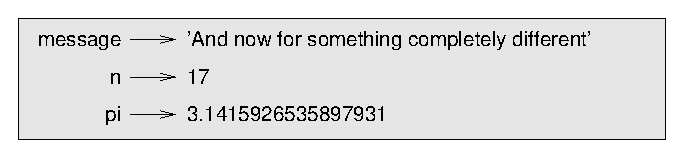
\includegraphics{figs/state2.eps}}
\afterfig

你可以使用一个print语句来显示变量的值:

\beforeverb
\begin{verbatim}
>>> print n
17
>>> print pi
3.14159265359
\end{verbatim}
\afterverb
%
一个变量的数据类型是这个变量对应值的数据类型。

\beforeverb
\begin{verbatim}
>>> type(message)
<type 'str'>
>>> type(n)
<type 'int'>
>>> type(pi)
<type 'float'>
\end{verbatim}
\afterverb
%
\begin{ex}
如果你在输入一个整数时以$0$开头,你会得到一个奇怪的错误:

\beforeverb
\begin{verbatim}
>>> zipcode = 02492
                  ^
SyntaxError: invalid token
\end{verbatim}
\afterverb

其他的数字也许可以工作,但是结果是诡异的:

\beforeverb
\begin{verbatim}
>>> zipcode = 02132
>>> print zipcode
1114
\end{verbatim}
\afterverb

你能指出这是为什么吗?提示:打印数值{\tt 01},{\tt 010},{\tt 0100}和{\tt 01000}。

\index{八进制}

\end{ex}

\section{变量命名和关键字}
\index{关键字}

程序员通常选取有意义的名字作为变量明——变量名说明了变量的作用。

变量名可以任意长。它们可以同时包含字母和数字,但必须以一个字母开头。大写字母的使用是合法的,但是一个好的习惯是使用小写字母作为变量的首字母(后面会说明原因)。

下划线符号(\verb"_")可以出现在一个变量名中,通常使用在有多个单词的名字中,如\verb"my_name"或者\verb"airspeed_of_unladen_swallow"。

\index{下划线字符}

如果你赋予了一个变量非法的名字,你会得到这样的一个语法错误:

\beforeverb
\begin{verbatim}
>>> 76trombones = 'big parade'
SyntaxError: invalid syntax
>>> more@ = 1000000
SyntaxError: invalid syntax
>>> class = 'Advanced Theoretical Zymurgy'
SyntaxError: invalid syntax
\end{verbatim}
\afterverb
%
{\tt 76trombones}是非法的,因为它不是有字母开始。{\tt more@}是非法的,因为它包含了非法字符{\tt @}。但是{\tt class}哪里错了呢?

事实上{\tt class}属于Python的一个{\bf 关键字}。解释器使用这些关键字来识别程序的结构,因此它们不能被用做变量名。

\index{关键字}

Python共有31个关键字\footnote{在Python 3.0中,{\tt exec}不再是一个关键字,但{\tt nonlocal}是。}:

\beforeverb
\begin{verbatim}
and       del       from      not       while    
as        elif      global    or        with     
assert    else      if        pass      yield    
break     except    import    print              
class     exec      in        raise              
continue  finally   is        return             
def       for       lambda    try
\end{verbatim}
\afterverb
%
你可以放一份关键字列表在手边。如果解释器报错说变量名有误,而你有不知道原因,看看这个变量名是否在关键字列表上。

\section{程序语句}

程序语句是一组Python解释器可以执行的代码。我们已经遇到过两种程序语句:print和assignment。

\index{程序语句}
\index{交互模式}
\index{脚本模式}

当你在交互模式下输入一条程序语句,解释器会执行该条语句,并显示结果,如果有结果的话。

一个脚本通常包含一系列程序语句。如果有多于一条程序语句,每执行一条语句将会显示对应的结果。

例如,脚本

\beforeverb
\begin{verbatim}
print 1
x = 2
print x
\end{verbatim}
\afterverb
%
会产生输出

\beforeverb
\begin{verbatim}
1
2
\end{verbatim}
\afterverb
%
赋值语句不产生输出。

\section{运算符和运算数}
\index{运算符,数学}
\index{数学运算符}
\index{运算数}
\index{表达式}

{\bf 运算符}是表示计算的特殊符号,如加法和乘法。运算符作用的数据被称为{\bf 运算数}。

运算符{\tt +}、{\tt -}、{\tt *}、{\tt /}和{\tt **}实现加法、减法、乘法、除法和指数运算,如下面的示例:

\beforeverb
\begin{verbatim}
20+32   hour-1   hour*60+minute   minute/60   5**2   (5+9)*(15-7)
\end{verbatim}
\afterverb
%
在一些其他的编程语言中,\verb"^"被用做指数运算,但是在Python中这是一个位操作,称为XOR。在本书中将不会涉及位操作的知识,你可以在\url{wiki.python.org/moin/BitwiseOperators}中阅读相关知识。

\index{位操作}
\index{运算符!按位}

%When a variable name appears in the place of an operand, it
%is replaced with its value before the operation is
%performed.

除法运算符有可能不按照你期望的运行:

\beforeverb
\begin{verbatim}
>>> minute = 59
>>> minute/60
0
\end{verbatim}
\afterverb
%
{\tt minute}的值是59,在传统的算术中,59除以60的结果是0.98333,而不是0。产生偏差的原因是因为Python执行了{\bf 下取整除法}\footnote{在Python 3.0中,这个除法的结果是一个{\tt 浮点数}。新的运算符{\tt //}执行取整除法。}。

\index{Python 3.0}
\index{下取整除法}
\index{浮点除法}
\index{除法!下取整}
\index{除法!浮点}

当两个运算数都是整数,结果同样是整数;下取整除法舍去了小数部分,因此在这个例子中结果为0。

如果任意一个运算数是一个浮点数,Python执行浮点除法,此时结果为{\tt 浮点数}:

\beforeverb
\begin{verbatim}
>>> minute/60.0
0.98333333333333328
\end{verbatim}
\afterverb


\section{表达式}

{\bf 表达式}是数值、变量和运算符的组合。一个数值是一个表达式,一个变量也是一个表达式,因此一下都是合法的表达式(假设变量{\tt x}已经被赋值):

\index{表达式}
\index{赋值}

\beforeverb
\begin{verbatim}
17
x
x + 17
\end{verbatim}
\afterverb
%
如果你在交互模式下输入一个表达式,解释器立即对它{\bf 赋值}并显示结果:

\beforeverb
\begin{verbatim}
>>> 1 + 1
2
\end{verbatim}
\afterverb
%
但在脚本中,一个表达式本身不做任何事情!初学者通常对此会产生困惑。

\begin{ex}
在交互模式下输入一下表达式,观察结果:

\beforeverb
\begin{verbatim}
5
x = 5
x + 1
\end{verbatim}
\afterverb
%
现在将这些表达式放在一个脚本文件里并运行。此时输出是什么?修改脚本,在每个表达式前添加print语句,然后观察输出。
\end{ex}


\section{运算符的优先级}
\index{运算符的优先级}
\index{优先级规则}
\index{PEMDAS}

当一个表达式中出现多于一个运算符时,求值的顺序由{\bf 优先级规则}决定。Python遵从数学运算符的约定。{\bf PEMDAS}是一个有效的方法来记忆这些规则:

\index{括号!压倒优先级}

\begin{itemize}

\item {\bf P}arentheses(括号)具有最高的优先级,可以强迫表达式按照指定的顺序求值。由于在括号中的表达式先被求值,{\tt 2 * (3-1)}的结果是4,{\tt (1+1)**(5-2)}的结果是8。你可以用括号来使得表达式更容易阅读,如{\tt (minute * 100) / 60},即便这并不改变最终的结果。

\item {\bf E}xponentiation(指数运算)有次高的优先级,因此{\tt 2**1+1}的结果是3,而不是4,{\tt 3*1**3}的结果是3,而不是27。

\item {\bf M}ultiplication(乘法)和{\bf D}ivision(除法)具有相同的优先级,并优于{\bf A}ddition(加法)和{\bf S}ubtraction(减法),它们同样具有相同的优先级。因此{\tt 6+4/2}的结果是8,而不是5。

\item 具有相同优先级的运算符是从左到右进行求值的。因此在表达式{\tt degrees / 2 * pi}中,首先计算除法,然后在结果上乘以{\tt pi}。如果要除以$2 \pi$,你需要使用括号,或者使用{\tt degrees / 2 / pi}。

\end{itemize}


\section{字符串操作}
\index{字符串!操作}
\index{运算符!字符串}

一般情况下,你不能使用算术运算符作用于字符串,即使字符串看起来像数字,因此以下是非法的:

\beforeverb
\begin{verbatim}
'2'-'1'    'eggs'/'easy'    'third'*'a charm'
\end{verbatim}
\afterverb
%
运算符{\tt +}可以作用于字符串,但未必按照你期望的方式工作:它执行的是{\bf 级联},即将字符串首尾相连。例如:

\index{级联}

\beforeverb
\begin{verbatim}
first = 'throat'
second = 'warbler'
print first + second
\end{verbatim}
\afterverb
%
程序的输出是{\tt throatwarbler}。

运算符{\tt *}同样可以作用于字符串,它的功能是重复字符串。如\verb"'Spam'*3"的结果是\verb"'SpamSpamSpam'"。如果一个运算符是字符串,那么另一个必须是一个整数。

运算符{\tt +}和{\tt *}在字符串的的使用类似加法和乘法,如{\tt 4*3}相当于{\tt 4+4+4},因此我们期望\verb"'Spam'*3"相当于\verb"'Spam'+'Spam'+'Spam'",事实如此。当然,字符串的级联和重复相比整数的加法和乘法还是有很大的区别的。你可以找出一个加法有而字符串级联没有的性质吗?


\index{交换性}


\section{注释}
\index{注释}

当程序变得越来越长,越来越复杂,它们变得更难读懂。正是的变成语言是密集的,通常很难通过阅读一小段代码来指出它是做什么的,或者为这么这么写。

由于这个理由,在程序旁添加标记,使用自然语言来说明这段程序是做什么的是一个良好的想法。这些标记被称为{\bf 注释},它们由\verb"#"符号开头:

\beforeverb
\begin{verbatim}
# compute the percentage of the hour that has elapsed
percentage = (minute * 100) / 60
\end{verbatim}
\afterverb
%
在这个例子中,注释以整行的方式出现。你也可以在一行的末尾添加注释:

\beforeverb
\begin{verbatim}
percentage = (minute * 100) / 60     # percentage of an hour
\end{verbatim}
\afterverb
%
{\tt \#}符号后到一行结束中的任何内容都被忽略---它们将不影响程序的运行。

当说明代码中不明显的特点时,注释非常有效。我们可以假设阅读代码的人可以指出代码{\em 做了什么};更有必要的是解释{\em 为什么这么做}。

以下的注释是冗余而无用的:

\beforeverb
\begin{verbatim}
v = 5     # assign 5 to v
\end{verbatim}
\afterverb
%
以下的注释包含了代码中没有的有用信息:

\beforeverb
\begin{verbatim}
v = 5     # velocity in meters/second. 
\end{verbatim}
\afterverb
%
好的变量明可以减少对注释的依赖,但长的变量名会使得表达式难以阅读,因此这是一个折衷。

\section{调试}
\index{调试}

目前位置你遇到的语法错误大多为非法变量明,如关键字{\tt class}和{\tt yield},或者包含非法字符,如\verb"odd~job"和\verb"US$"。

\index{语法错误}
\index{错误!语法}

如果你在一个变量名中加入一个空格,Python会认为这是两个没有运算符的运算数:

\beforeverb
\begin{verbatim}
>>> bad name = 5
SyntaxError: invalid syntax
\end{verbatim}
\afterverb
%
对于语法错误,错误消息没有很大的帮助。通常的消息是{\tt SyntaxError: invalid syntax}和{\tt SyntaxError: invalid token},它们都不包含很多信息量。

\index{错误消息}
\index{未定义而使用}
\index{异常}
\index{运行时错误}
\index{错误!运行时}

运行时错误通常由于“未定义而使用”,即试图使用一个没有赋值的变量。这会在你拼写变量名错误时发生:

\beforeverb
\begin{verbatim}
>>> principal = 327.68
>>> interest = principle * rate
NameError: name 'principle' is not defined
\end{verbatim}
\afterverb
%
变量名是大小写敏感的,因此{\tt LaTeX}和{\tt latex}是不同的。

\index{大小写敏感,变量名}
\index{语义错误}
\index{错误!语义}

语义错误通常发生在运算符的顺序上。例如,求值$\frac{1}{2 \pi}$,你也许会写成:

\beforeverb
\begin{verbatim}
>>> 1.0 / 2.0 * pi
\end{verbatim}
\afterverb
%
但是首先执行了除法,因此你会得到$\pi / 2$,并不是想要的结果!Python没有办法知道你写的是什么含义,因此这种情况下你不会得到一个错误消息;你得到的只是错误的结果。

\index{运算符优先级}

\section{术语表}

\begin{description}

\item[数值:] 程序操作的基本数据单元,如一个数字或字符串。
\index{数值}

\item[类型:] 数据的分类。目前为止我们见过的类型有整数({\tt int}),浮点数({\tt float}),和字符串({\tt str})。
\index{类型}

\item[整数:] 表示所有整数的类型。
\index{整数}

\item[浮点数:] 表示具有小数部分的数的类型。
\index{浮点数}

\item[字符串:] 表示一串字符的数据类型。
\index{字符串}

\item[变量:] 指向一个数值的名称。
\index{变量}

\item[语句:] 一段代表命令或行为的代码。目前为止我们见过的语句有赋值语句和打印语句。
\index{语句}

\item[赋值:] 将数值赋值给变量的语句。
\index{赋值}

\item[状态图:] 表示变量和对应数值的图。
\index{状态图}

\item[关键字:] 一些编译器用来对程序进行语法分析的保留单词,你不能使用例如{\tt if},{\tt  def}和{\tt while}作为变量名。
\index{关键字}

\item[运算符:] 表示一种简单运算的特殊符号,如加法,乘法,或者字符串级联。
\index{运算符}

\item[运算数:] 运算符作用的数值。
\index{运算数}

\item[下取整除法:] 两数相除并舍去小数部分的运算。
\index{下取整除法}

\item[表达式:] 表示单一结果的变量、运算符和数值的组合。
\index{表达式}

\item[求值] 通过执行运算符化简表达式得到一个单一结果。

\item[优先级规则] 定义运算符和运算数求值顺规的规则。
\index{优先级规则}
\index{优先级}

\item[级联:] 将两个运算数首尾现连。
\index{级联}

\item[注释:] 程序中提供给程序员(或者任何阅读程序的人)信息,但不影响程序执行的内容。
\index{注释}

\end{description}


\section{练习}

\begin{ex}
假设我们执行了如下的赋值语句:

\begin{verbatim}
width = 17
height = 12.0
delimiter = '.'
\end{verbatim}

对于下列表达式,写出表达式的数值和数据类型(表达式的数值)。

\begin{enumerate}

\item {\tt width/2}

\item {\tt width/2.0}

\item {\tt height/3}

\item {\tt 1 + 2 * 5}

\item {\tt delimiter * 5}

\end{enumerate}

使用Python解释器来验证你的结果。
\end{ex}

\begin{ex}
练习使用Python解释器作为计算器。
\index{calculator}

\begin{enumerate}

\item 一个半径为$r$的球的体积为$\frac{4}{3} \pi r^3$。一个半径为5的球体的体积是多少?提示:392.6是错误的!

\item 假设一本书的封面价格是\$24.95,书店提供40\%的折扣,对第一本书的运输费用为\$3,往后每增加一本需要75每分,如果购买60本书总共需要多少?

\item 如果我在6:52离开我家,用轻松的步伐跑了1英里(8:15每英里),然后保持节奏跑了3英里(7:12每英里),最后用轻松的步伐跑了1英里,我什么时候回到家吃早饭?

\index{跑步比赛}

\end{enumerate}
\end{ex}


\chapter{函数}
\label{funcchap}
\index{function call 函数调用}

在程序设计中,函数是带有函数名的一系列执行计算的语句,当定义一个函数,我们指
定一个函数名和一系列的语句。然后,就可以通过函数名调用函数。我们其实已经看到
一个函数调用的例子。

\beforeverb
\begin{verbatim}
>>>type(32)
<type 'int'>
\end{verbatim}
\afterverb

函数名是类型,小括号里的表达式称作函数的形式参数(argument).结果是形参的类型。

\index{parenthess!argument in}

通常我们这么说:函数接受一个参数,返回一个结果(叫做返回值)。

\index{argument 形式参数}
\index{return value 返回值}

\section{类型转换函数}
\index{conversion!type 转换!类型}
\index{type conversion 类型转换}

Python提供一些内置函数用来把一种类型的值转换成另一类型。{\\t int}函数接受一
个值,如果可以,就把它转换成整数,否则就会“抱怨”。

\index{int function int 函数}
\index{function!int 函数!int}

\beforeverb
\begin{verbatim}
>>> int('32')
32
>>> int('Hello')
Traceback (most recent call last):
  File "<stdin>", line 1, in <module>
ValueError: invalid literal for int() with base 10: 'Hello'
\end{verbatim}
\afterverb

{\tt int}函数可以把浮点数转换为整数,但是不能向上取整,只能截掉小数部分:

\beforeverb
\begin{verbatim}
>>> int(3.99999)
3
>>> int(-2.3)
-2
\end{verbatim}
\afterverb

{\tt float}函数把整数和字符串转换成浮点数:

\index{float function float函数}
\index{function!float 函数!float}

\beforeverb
\begin{verbatim}
>>>float(32)
32.0
>>>float('3.14159')
3.14159
\end{verbatim}
\afterverb \footnote{在译者的机器上float('3.14159')的输出为:3.1415899999999999(解释器Python2.5和2.6);3.14159(解释器Python3.1)。}

最后,{\tt str}把参数转换为字符串:

\index{str function str函数}
\index{function!str 函数!str}

\beforeverb
\begin{verbatim}
>>>str(32)
'32'
>>>str(3.14159)
'3.14159'
\end{verbatim}
\afterverb

2236




\chapter{实例学习:接口设计}


\chapter{条件语句和递归}

\section{ 模操作符}

\index{modulus operator 模操作符}
\index{operator!modulus 操作符!模}

模操作符用于两个整数,第一个操作数除以第二个操作数产生余数。在Python
中,模操作符是一个百分号(\verb"%")。语法的格式和其他的操作符相同。

\beforeverb
\begin{verbatim}
>>>quotient = 7 / 3
>>>print quotient
2
>>>remainder = 7 % 3
>>>print remainder
1
\end{verbatim}
\afterverb

7除以3等于2余1。\\

模操作符是非常有用的,比如,你可以查看一个数是否可以被另一个数整除---
如果{\tt x \% y}是0,{\tt x}就可以被{\tt y}整除。\\

\index{divisibility 整除}

你也可以用模运算来提取整数的最右边的数字。比如,{\tt x \% 10 }得到{\tt x}的最右面的一个数字\footnote{译注:个位数}(以十为底)。类似地,
{\tt x \% 100}得到最后的两位数字\footnote{十位和个位的数字}。

\section{布尔表达式}
\index{boolean expression 布尔表达式}
\index{expression!boolean}
\index{logical operator 逻辑运算符}
\index{operator!logical}

布尔表达式的结果要么是真(true),要么为假(false)。下面的例子是使用
{\tt ==}运算符,比较两个操作数,如果相等则结果为{\tt True},否则为{\tt False}:

\beforeverb
\begin{verbatim}
>>> 5 == 5
True
>>> 5 == 6
False
\end{verbatim}
\afterverb

{\tt True}和{\tt False}是两个特殊的值,属于{\tt bool}类型;他们不是
字符串:

\index{True special value True特殊值}
\index{False special value False特殊值}
\index{specail value!True}
\index{special value!False}
\index{bool type bool类型}
\index{type!bool}

\beforeverb
\begin{verbatim}
>>> type(True)
<type 'bool'>
>>> type(False)
<type 'bool'>
\end{verbatim}
\afterverb

{\tt ==}运算符是关系运算符中的一个,其他的还有:

\beforeverb
\begin{verbatim}
      x != y               # x is not equal to y
      x > y                # x is greater than y
      x < y                # x is less than y
      x >= y               # x is greater than or equal to y
      x <= y               # x is less than or equal to y
\end{verbatim}
\afterverb


尽管你可能很熟悉这些运算符,他们在Python中的表示方法和数学中的有很大
的不同。一个常见的错误是只使用一个{\tt =}号,而不是两个{\tt ==}号。
记住{\tt =}是赋值操作符,{\tt ==}是关系运算符。而且,Python中没有这样
的符号{\tt =<}或者{\tt =>}\footnote{在FP(functional programming中可能
会遇到这个符号}。

\index{relational operator 关系运算符}
\index{operator!relational}

\section{逻辑运算符}
\index{logical operator 逻辑运算符}
\index{operator!logical}

有三个逻辑运算符:{\tt and},{\tt or}和{\tt not}。这些操作符的意思和
在英语中的意思差不多。比如,{\tt x > 0 and x < 10}为真,仅当{\tt x}
大于0小于10\footnote{译注:在Python中,更pythonic的写法是 0 < x < 10
。  这样的符号对于c/c++背景的程序员来说,有点陌生,在c/c++等值的分别
是\&\&, || ,!}。

\index{and operator and运算符}
\index{or operator or运算符}
\index{not operator not运算符}
\index{operator!and}
\index{operator!or}
\index{operator!not}





\chapter{ “结果”函数}

\label{fruitchap}

\section{返回值}
\index{返回值}

我们使用的一些内建函数,如数学函数,会返回结果。调用这些函数的过程中会产生一个数值,通常我们将它赋值给一个变量,或者作为表达式的一部分。

\beforeverb
\begin{verbatim}
e = math.exp(1.0)
height = radius * math.sin(radians)
\end{verbatim}
\afterverb
%
目前为止我们所写的函数都是空的:它们打印一些东西或者移动乌龟,但它们的返回值都是{\tt 空}。

在本章中,我们开始编写卓有成效的函数。第一个例子是{\tt area},它返回给定半径的圆的面积:

\beforeverb
\begin{verbatim}
def area(radius):
    temp = math.pi * radius**2
    return temp
\end{verbatim}
\afterverb
%
我们先前见过  {\tt return} 语句,但在卓有成效的函数中, {\tt return} 语句包含一个表达式。返回语句的含义为:“立即从函数返回,并将表达式的值作为返回值”。表达式可以任意复杂,因此我们可以这样更简洁的写这个函数:

\index{返回语句}
\index{语句!返回}

\beforeverb
\begin{verbatim}
def area(radius):
    return math.pi * radius**2
\end{verbatim}
\afterverb
%
同时,{\bf 临时变量} 如 {\tt temp} 通常使得调试更为方便。

\index{临时变量}
\index{变量!临时}

有时一个函数会有多个返回语句,每一条位于一个条件分支中:

\beforeverb
\begin{verbatim}
def absolute_value(x):
    if x < 0:
        return -x
    else:
        return x
\end{verbatim}
\afterverb
%
由于 {\tt return} 语句位于一个选择的条件中,只有一条会被执行。

当一条返回语句被执行时,函数立刻返回,而不再执行后面的语句。在 {\tt return} 语句后的代码,或者存在于任何程序流执行不到的地方的代码,称为 {\bf 死区代码}。

\index{死区代码}

在一个卓有成效的函数中,确保每个可能的路径都对应一个{\tt return} 语句是一个良好的习惯。例如:

\beforeverb
\begin{verbatim}
def absolute_value(x):
    if x < 0:
        return -x
    if x > 0:
        return x
\end{verbatim}
\afterverb
%
这个程序是错误的,因为当 {\tt x} 恰为0的时候,没有一个条件语句为真,函数结束时没有遇到{\tt return} 语句。如果一个程序执行到函数的末尾,它将返回一个 {\tt None}值,而不是绝对值0.

\index{None特殊值}
\index{特殊值!None}

\beforeverb
\begin{verbatim}
>>> print absolute_value(0)
None
\end{verbatim}
\afterverb
%
顺便一提,Python提供了一个内建函数{\tt abs},可以计算一个数的绝对值。

\index{绝对值函数}
\index{函数!绝对值}

\begin{ex}

\index{比较函数}
\index{函数!比较}

编写 {\tt 比较} 函数,函数返回 {\tt 1} 如果 {\tt x > y},返回{\tt 0} 如果 {\tt x == y},返回 {\tt -1} 如果 {\tt x < y}。
\end{ex}


\section{增量开发}
\label{增量开发}
\index{开发计划!增量}

当你编写越来越大的函数时,你发现在调试上会花更多的时间。

对于越加复杂的程序,你可以尝试{\bf 增量开发}的方法。增量开发是通过每次测试一小部分代码的方法来避免过长的调试过程。

\index{测试!增量开发}
\index{毕达哥拉斯理论}

例如,假设你需要计算给定坐标$(x_1, y_1)$和$(x_2, y_2)$两点间的距离。根据毕达哥拉斯理论,距离为:

\begin{displaymath}
\mathrm{distance} = \sqrt{(x_2 - x_1)^2 + (y_2 - y_1)^2}
\end{displaymath}
%
首先考虑 {\tt distance} 函数在Python中应该是如何的。换言之,函数的输入(参数)和输出(返回值)应该是什么?

在本例中,输入是两个点,你可以用4个数来表示。返回值是距离,可以用一个浮点数来表示。

现在你可以写出函数的框架:

\beforeverb
\begin{verbatim}
def distance(x1, y1, x2, y2):
    return 0.0
\end{verbatim}
\afterverb
%
显然,这个版本并没有计算距离;它总是返回零。但是它的语法是正确的,可以正常运行,这意味着你在把它修改的更复杂前可以测试它。

为了测试新函数,我们使用样例参数来调用它:

\beforeverb
\begin{verbatim}
>>> distance(1, 2, 4, 6)
0.0
\end{verbatim}
\afterverb
%
我选择的两个点水平距离为3,垂直距离为4,因此两点距离为5(斜边为3-4-5的三角形)。当测试一个函数时,直到正确答案是很有用的。

\index{测试!直到答案}

现在我们确定函数的语法是正确的,我们可以开始添加代码。下一步是计算$x_2 - x_1$ 和 $y_2 - y_1$的差,下一个版本将这两个值储存在临时变量中,并打印。

\beforeverb
\begin{verbatim}
def distance(x1, y1, x2, y2):
    dx = x2 - x1
    dy = y2 - y1
    print 'dx is', dx
    print 'dy is', dy
    return 0.0
\end{verbatim}
\afterverb
%
如果函数可以工作,它应该显示 \verb"'dx is 3'" 以及 {\tt 'dy is 4'}。如果没错,我们知道函数得到了正确的参数,并正确的执行了第一步计算。如果有错,我们只需要检查几行代码。

下一步我们计算 {\tt dx} 和 {\tt dy}的平方和:

\beforeverb
\begin{verbatim}
def distance(x1, y1, x2, y2):
    dx = x2 - x1
    dy = y2 - y1
    dsquared = dx**2 + dy**2
    print 'dsquared is: ', dsquared
    return 0.0
\end{verbatim}
\afterverb
%
同样,你可以运行程序,并检查结果(应该是25)。最后你可以使用 {\tt math.sqrt} 来计算并返回结果。

\index{开根}
\index{函数!开根}

\beforeverb
\begin{verbatim}
def distance(x1, y1, x2, y2):
    dx = x2 - x1
    dy = y2 - y1
    dsquared = dx**2 + dy**2
    result = math.sqrt(dsquared)
    return result
\end{verbatim}
\afterverb
%
如果运行正确,你就完成了这个程序。否则,你需要在返回语句前打印 {\tt result}。

函数的最终版本在执行过程中并不显示任何内容。{\tt print}语句在调试的过程中非常有用,但是一旦程序工作正常了,你需要删除它们。这样的代码被称为{\bf 脚手架代码},它们对编写程序有帮助,但并不是最终结果的一部分。

\index{脚手架代码}

当你刚开始时,你应该每次只添加几行代码。当你变得熟练时,你发现你可以调试大段的代码。通常,增量开发可以节约你很多调试的时间。

这个过程的关键在于:

\begin{enumerate}

\item 编写程序时每次只做少量修改,在任何时刻如果出错,你可以很方便的定位错误。

\item 使用临时变量记录中间过程值,这样你可以显示并检查它们。

\item 当程序正常工作后,你可能需要删除一些脚手架代码或者合并多个语句为一个复合语句。注意保持程序的可读性。

\end{enumerate}

\begin{ex}

\index{斜边}

使用增量开发编写一个 {\tt 斜边} 函数,读取三角形两条直角边作为参数,返回斜边长度。记录下开发过程中的每一个阶段。
\end{ex}

\section{Composition}

\index{复合}
\index{函数复合}

现在你应该可以预料,你可以在一个函数中调用另一个函数。这种能力被称为 {\bf 复合}。

例如,我们将写一个函数,它读入两个点作为参数,一个是圆心,另一个是圆周上的一个点,该函数将计算圆周的面积。

假设圆心对应的点保存在变量 {\tt xc} 和{\tt yc},圆周上的点的坐标为 {\tt xp} 和 {\tt yp}。第一步是计算圆的半径,即两点之间的距离。我们刚写了函数 {\tt distance},它实现了这个功能:

\beforeverb
\begin{verbatim}
radius = distance(xc, yc, xp, yp)
\end{verbatim}
\afterverb
%
第二部是通过半径计算圆的面积,我们刚才也实现了:

\beforeverb
\begin{verbatim}
result = area(radius)
\end{verbatim}
\afterverb
%
将这两步封装在一个函数,我们得到:

\index{封装}

\beforeverb
\begin{verbatim}
def circle_area(xc, yc, xp, yp):
    radius = distance(xc, yc, xp, yp)
    result = area(radius)
    return result
\end{verbatim}
\afterverb
%
临时变量 {\tt radius} 和 {\tt result} 用来开发和调试,但是当程序正常工作后,我们可以通过复合这些函数调用来使得程序看起来更简洁:

\beforeverb
\begin{verbatim}
def circle_area(xc, yc, xp, yp):
    return area(distance(xc, yc, xp, yp))
\end{verbatim}
\afterverb
%

\section{布尔函数}
\label{布尔}

\index{布尔函数}

函数可以返回布尔值,这样便于隐藏函数中复杂的细节。例如:

\beforeverb
\begin{verbatim}
def is_divisible(x, y):
    if x % y == 0:
        return True
    else:
        return False
\end{verbatim}
\afterverb
%
通常布尔函数的函数名类似yes/no的问题; \verb"is_divisible" 根据{\tt x}是否可以被{\tt y}整除,返回 {\tt True} 或 {\tt False}。

下面给出一个例子:

\beforeverb
\begin{verbatim}
>>>   is_divisible(6, 4)
False
>>>   is_divisible(6, 3)
True
\end{verbatim}
\afterverb
%
运算符 {\tt ==} 的结果返回一个布尔值,所以我们可以直接返回结果,这样更加简洁:

\beforeverb
\begin{verbatim}
def is_divisible(x, y):
    return x % y == 0
\end{verbatim}
\afterverb
%
布尔函数通常用在条件语句中:

\index{条件语句}
\index{语句!条件}

\beforeverb
\begin{verbatim}
if is_divisible(x, y):
    print 'x is divisible by y'
\end{verbatim}
\afterverb
%
也许会写成类似如下的代码:

\beforeverb
\begin{verbatim}
if is_divisible(x, y) == True:
    print 'x is divisible by y'
\end{verbatim}
\afterverb
%
但是多余的比较是不必要的。

\begin{ex}
写一个函数 \verb"is_between(x, y, z)" ,如果$x \le y \le z$则返回 {\tt True},否则返回 {\tt False} 。
\end{ex}


\section{更多递归}

\index{递归}
\index{图灵完备语言}
\index{语言!图灵完备}
\index{Turing, Alan}
\index{图灵理论}

我们仅仅覆盖了Python的一小部分,但也许你会对这是一个{\em 完备}的编程语言集感兴趣,即任何可以被计算的东西都可以用这用语言来表示。任何现有的程序都可以用你现在学到的语言特征重写(事实上你还需要一些命令来控制键盘、鼠标、磁盘等设备,但仅此而已)。

这种说法首先由早期计算机科学家Alan Turing提出(有人会争论他是一个数学家,但许多早期的计算机科学家是数学家起家的),被称为图灵理论。如果你想对图灵理论有更完全(更精确)的讨论,我推荐Michael Sipser's的书 {\em Introduction to the Theory of Computation}。

为了让你认识到你可以用到目前为止学到的工具做什么,我们来计算一些递归定义的数学函数。递归定义类似循环定义,定义的本身包含对所定义的东西的引用。一个真正的循环定义不是很有用:

\begin{description}

\item[frabjous:] 一个描述frabjous东西的形容词。

\end{description}

\index{frabjous}
\index{循环定义}
\index{定义!循环}

如果在字典里看到这样的解释,你也许会感到恼怒。然而,如果你查看阶乘的定义(表示为$!$),你会的到类似这样的东西:

\vspace{-0.35in}
\begin{eqnarray*}
&&  0! = 1 \\
&&  n! = n (n-1)!
\end{eqnarray*}
\vspace{-0.25in}

这个定义规定0的阶乘是1,对于其他的任何数 $n$的阶乘,其值为 $n$ 乘以 $n-1$的阶乘。

因此 $3!$ 的阶乘是 3 乘以 $2!$,$2!$的阶乘是  2 乘以 $1!$,$1!$的阶乘是 1 乘以$0!$。将这些放在一起,$3!$ 等于3乘以2乘以1乘以1,结果为6。

\index{阶乘函数}
\index{函数!阶乘}
\index{递归定义}

如果你可以写出某个东西的递归定义,你通常可以通过写一个Python程序来进行求值。第一步是决定参数。很明显在本例中 {\tt factorial} 读取一个整数作为参数:

\beforeverb
\begin{verbatim}
def factorial(n):
\end{verbatim}
\afterverb
%
如果参数等于0,我们所要做的就是返回1:

\beforeverb
\begin{verbatim}
def factorial(n):
    if n == 0:
        return 1
\end{verbatim}
\afterverb
%
否则,将开始有趣的部分,我们递归的调用阶乘函数 $n-1$ 然后乘以$n$:

\beforeverb
\begin{verbatim}
def factorial(n):
    if n == 0:
        return 1
    else:
        recurse = factorial(n-1)
        result = n * recurse
        return result
\end{verbatim}
\afterverb
%
程序的执行流程类似章节~\ref{递归}中 {\tt countdown} 。如果我们使用参数3调用 {\tt factorial}:

由于3不是0,我们得到第二个计算{\tt n-1}阶乘的分支...

\begin{quote}
由于2不是0,我们得到第二个计算{\tt n-1}阶乘的分支...


  \begin{quote}
  由于1不是0,我们得到第二个计算{\tt n-1}阶乘的分支...


    \begin{quote}
    由于0{\em 等于}0,我们得到第一个分支,返回结果1,不再进行更多的递归调用。
    \end{quote}


  返回值(1)被乘以 $n$,对应1,然后结果返回。
  \end{quote}


返回值(1)被乘以 $n$,对应2,然后结果返回。 
\end{quote}


返回值(2)被乘以 $n$,对应3,结果为6,这是整个函数最终返回的结果。

\index{栈图}
下面给出这一系列函数调用对应的栈图:

\vspace{0.1in}
\beforefig
\centerline{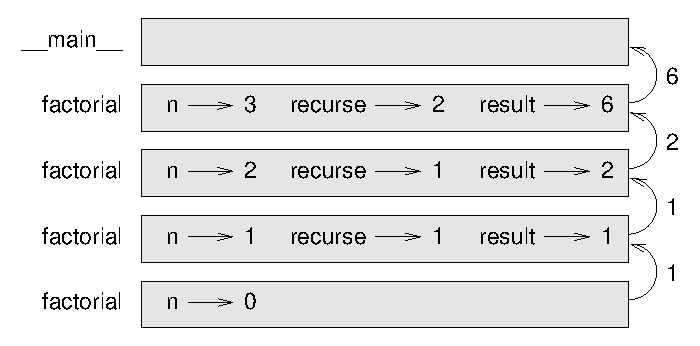
\includegraphics{figs/stack3.eps}}
\afterfig
\vspace{0.1in}

如图所示,返回值通过栈向上传递。在每一帧中,返回值是{\tt result}的值,即 {\tt n} 和 {\tt recurse}的乘积。

\index{帧}

在最后一帧中,局部变量 {\tt recurse} 和 {\tt result} 并不存在,因为该分支并没有创建它们。


\section{信心的飞跃}
\index{递归}
\index{信心的飞跃}

按照程序执行流程是阅读程序的一个方法,但这么做很容易走入迷宫。这里给出另一个方法,我称之为“信心的飞跃”。当你遇到一个函数调用,你{\em 假设}函数执行无误,并返回正确的结果,而不是追溯程序执行流程。

事实上,当你调用内建函数时,你已经体验过信心的飞跃。当你调用 {\tt math.cos} 和 {\tt math.exp}时,你并不检查这些函数的主体。你仅仅假设它们是由优秀的程序员编写的,可以正常的工作。

这同样适用于你自己写的函数。例如,在章节~\ref{布尔}中,我们编写了一个叫做\verb"is_divisible"的函数,判断一个数是否可以被另一个数整除。一旦我们通过检查测试函数确信它可以正常工作,我们可以直接调用该函数,而不用再去查看函数主体。

\index{测试!信心的飞跃}

以上思想同样适用于递归程序。当你遇到递归调用,你应该假设递归调用工作正常(并返回正确结果),而不是跟着程序执行流程。你可以这么问你自己,“假设我可以得到$n-1$的阶乘,我应该怎么计算$n$的阶乘?”很明显,通过乘以$n$就可以了。

当然,假设程序工作正常,而事实上你还没有完成这个函数,这里有一些诡异,但这就是为什么称之为信心的飞跃!


\section{另一个例子}
\label{另一个例子}

\index{斐波纳契函数}
\index{函数!斐波纳契}

除了 {\tt 阶乘}外,最常见的递归定义的数学函数是 {\tt 斐波纳契}函数,其定义如下:\footnote{参见 \url{wikipedia.org/wiki/Fibonacci_number}。}:

\vspace{-0.25in}
\begin{eqnarray*}
&& \mathrm{fibonacci}(0) = 0 \\
&& \mathrm{fibonacci}(1) = 1 \\
&& \mathrm{fibonacci}(n) = \mathrm{fibonacci}(n-1) + \mathrm{fibonacci}(n-2);
\end{eqnarray*}
%
翻译成Python为:

\beforeverb
\begin{verbatim}
def fibonacci (n):
    if n == 0:
        return 0
    elif  n == 1:
        return 1
    else:
        return fibonacci(n-1) + fibonacci(n-2)
\end{verbatim}
\afterverb
%
如果你试图跟随执行过程,即使很小的数$n$,你的脑袋也会爆炸。但是根据信心的飞跃,假设两个递归调用工作正确,就很容易看出通过将两者相加你将得到正确的结果。

\index{执行流程}


\section{类型检查}
\label{监护人}

\index{类型检查}
\index{错误检查}
\index{阶乘函数}

如果我们调用 {\tt factorial} 函数时提供的参数是1.5会怎么样?

\index{运行时错误}

\beforeverb
\begin{verbatim}
>>> factorial(1.5)
RuntimeError: Maximum recursion depth exceeded
\end{verbatim}
\afterverb
%
看起来这将会是一个无穷的递归。这事怎么发生的?递归函数有一个初始情况————当 {\tt n == 0}。但是如果 {\tt n} 不是一个整数,我们将 {\em 错过} 初始状态并不断的递归。

\index{无穷递归}
\index{递归!无穷}

在第一次递归调用中, {\tt n} 的值是0.5。在下一次调用时,它变为 -0.5。接着,它变得越来越小(更朝负方向),永远不会为0。

我们有两种选择。我们可以推广 {\tt factorial}函数使之可以工作在浮点数,或者我们可以让 {\tt factorial} 检查参数的数据类型。第一个方法可以参考gamma函数\footnote{参考 \url{wikipedia.org/wiki/Gamma_function}。},超出了本书的范围。让我们看看第二个方法。

\index{gamma函数}

我们可以使用内建函数 {\tt isinstance} 来验证参数的数据类型。同时我们可以确保参数的正的:

\index{isinstance函数}
\index{函数!isinstance}

\beforeverb
\begin{verbatim}
def factorial (n):
    if not isinstance(n, int):
        print 'Factorial is only defined for integers.'
        return None
    elif n < 0:
        print 'Factorial is only defined for positive integers.'
        return None
    elif n == 0:
        return 1
    else:
        return n * factorial(n-1)
\end{verbatim}
\afterverb
%
第一部分处理非整数;第二部分捕获负数。在这两种情况下程序将打印错误信息,并返回 {\tt None}表示有错误发生:

\beforeverb
\begin{verbatim}
>>> factorial('fred')
Factorial is only defined for integers.
None
>>> factorial(-2)
Factorial is only defined for positive integers.
None
\end{verbatim}
\afterverb
%
如果通过了两个检查,我们知道 $n$ 是一个正整数,可以保证递归会终止。

\index{守护人模式}
\index{模式!监护人}

这个程序展示了一个称为{\bf 监护人}的模式。前两个条件扮演了监护人的角色,防止错误的参数造成代码运行的错误。监护代码保证了程序的正确性。


\section{调试}
\label{factdebug}

\index{调试}

将大的程序拆成小的函数的过程给出了合理的调试测试点。如果一个函数工作不正常,有三种情况需要考虑:

\begin{itemize}

\item 函数得到的参数有误,即先决条件没有满足。

\item 函数本身有误,即后决条件没有满足。

\item 返回之有误,或者使用方式不正确。

\end{itemize}

为了排除第一种可能性,你可以在函数开始部分添加{\tt print}语句,打印参数值(数据类型)。或和你可以直接编写代码检查先决条件。

\index{先决条件}
\index{后决条件}

如果参数没有问题,在每条{\tt return}语句前添加{\tt print}语句,打印返回值。可能的话手工检查结果。试图使用容易检查的参数来调用函数(参见章节~\ref{增量开发})。

如果函数工作正常,检查函数调用,确保返回值被正确使用(或被使用!)。

\index{执行流程}

在函数开始和结尾添加打印语句可以使程序流程更加明显。例如,下面给出带打印语句的{\tt factorial}函数:

\beforeverb
\begin{verbatim}
def factorial(n):
    space = ' ' * (4 * n)
    print space, 'factorial', n
    if n == 0:
        print space, 'returning 1'
        return 1
    else:
        recurse = factorial(n-1)
        result = n * recurse
        print space, 'returning', result
        return result
\end{verbatim}
\afterverb
%
{\tt space}是空格的字符串,用来缩进输出结果。下面给出{\tt factorial(5)}的输出结果:

\beforeverb
\begin{verbatim}
                     factorial 5
                 factorial 4
             factorial 3
         factorial 2
     factorial 1
 factorial 0
 returning 1
     returning 1
         returning 2
             returning 6
                 returning 24
                     returning 120
\end{verbatim}
\afterverb
%
如果你不清楚程序执行的流程,这样的输出信息很有帮助。搭建脚手架会花费一些时间,但会帮助节省很多调试时间。


\section{术语}

\begin{description}

\item[临时变量:] 在复杂的计算过程中用来记录中间值的变量。
\index{临时变量}
\index{变量!临时}

\item[死区代码:] 程序中无法执行到的代码,通常因为出现在 {\tt return} 语句的后面。
\index{死区代码}

\item[{\tt None}:]  一个特殊的函数返回值,表明函数没有返回语句,或者返回语句没有参数。
\index{None特殊值}
\index{特殊值!None}

\item[增量开发:] 一种程序开发的方法,通过每次添加测试少量代码来避免程序的调试。
\index{增量开发}

\item[脚手架:] 在程序开发过程中使用的代码,并不出现在最终版本中。
\index{脚手架}

\item[守护人:] 使用条件语句检查错误并处理可能出错的情况的编程模式。
\index{守护人模式}
\index{模式!守护人}

\end{description}


\section{练习}

\begin{ex}
\index{栈图}

画下面程序的栈图。程序执行时会打印什么内容?

\beforeverb
\begin{verbatim}
def b(z):
    prod = a(z, z)
    print z, prod
    return prod

def a(x, y):
    x = x + 1
    return x * y

def c(x, y, z):
    sum = x + y + z
    pow = b(sum)**2
    return pow

x = 1
y = x + 1
print c(x, y+3, x+y)
\end{verbatim}
\afterverb

\end{ex}


\begin{ex}
\index{Ackerman函数}
\index{函数!ack}

Ackermann函数,$A(m, n)$,定义为\footnote{See \url{wikipedia.org/wiki/Ackermann_function}。}:

\begin{eqnarray}
A(m, n) = \begin{cases} 
              n+1 & \mbox{if } m = 0 \\ 
        A(m-1, 1) & \mbox{if } m > 0 \mbox{ and } n = 0 \\ 
A(m-1, A(m, n-1)) & \mbox{if } m > 0 \mbox{ and } n > 0.
\end{cases} 
\end{eqnarray}
%
编写一个 {\tt ack}的函数来计算 Ackerman's 公式。使用你的函数来计算 {\tt ack(3, 4)},结果应该是125。如果选择大的 {\tt m} 和 {\tt n}会发生什么?

\end{ex}


\begin{ex}
\label{回文}

\index{回文}

回文是一个从前往后和从后往前拼写相同的单词,如“noon”和“redivider”。从递归的角度来看,如果一个单词第一个字母和最后一个字母相同,且中间是回文的,那么这个单词是回文的。

下面的函数读取一个字符串作为参数,分别返回第一个、最后一个和中间的字母:

\beforeverb
\begin{verbatim}
def first(word):
    return word[0]

def last(word):
    return word[-1]

def middle(word):
    return word[1:-1]
\end{verbatim}
\afterverb
%
我们会在章节~\ref{strings}学习它们是如何工作的。

\begin{enumerate}

\item 在{\tt palindrome.py}文件中输入这些函数并测试。如果你输入两个字母,调用{\tt middle}会返回什么?一个字母呢?空字符串呢(使用\verb"''"输入,不包含任何字母)?

\item 编写函数\verb"is_palindrome",读取一个字符串作为参数,如果是回文则返回{\tt True},否则返回{\tt False}。你可以使用内建的{\tt len}函数来检查字符串的长度。

\end{enumerate}

\end{ex}

\begin{ex}
数$a$称为数$b$的幂,如果$a$可以被$b$整除,同时$a/b$是$b$的幂。编写函数\verb"is_power",读取{\tt a}和{\tt b}作为参数,如果{\tt a}是{\tt b}的幂则返回{\tt True}。
\end{ex}


\begin{ex}

\index{最大公约数(GCD)}
\index{GCD(最大公约数)}

最大公约数(GCD)是可以整除$a$和$b$最大的书\footnote{本练习基于Abelson and Sussman's {\em Structure and Interpretation of Computer Programs}的习题。}。

寻找两个数的GCD的一个方法是欧几里得算法,算法指出如果$r$是$a$除以$b$的余数,那么$gcd(a, b) = gcd(b, r)$。对于基本情况,我们考虑$gcd(a, 0) = a$。

\index{欧几里得算法}
\index{算法!欧几里得}

编写函数\verb"gcd" ,参数为{\tt a}和{\tt b},返回值为两者的最大公约数。如果你需要帮助,参考\url{wikipedia.org/wiki/Euclidean_algorithm}。

\end{ex}



\chapter{迭代}


\chapter{字符串}
\label{字符串}


\section{字符串是一个序列}
\index{序列}
\index{字符}
\index{括号运算符}
\index{运算符!括号}

字符串是字符的 {\bf 序列} 。你可以使用括号运算符每次访问一个字符。 

\beforeverb
\begin{verbatim}
>>> fruit = 'banana'
>>> letter = fruit[1]
\end{verbatim}
\afterverb
%
第二条语句从{\tt fruit}中读取第一个字符,并赋值给{\tt letter}。

\index{下标}

在括号中的表达式称为{\bf 下标}。下标指示了序列中对应的字符。

但是你也许没有得到你期望的:

\beforeverb
\begin{verbatim}
>>> print letter
a
\end{verbatim}
\afterverb
%
对于大多数人来说,\verb"'banana'"是{\tt b},而不是{\tt a}。但是对计算机科学家来说,下标是从字符串开始位置的偏移量,第一个字符的偏移量是零。

\beforeverb
\begin{verbatim}
>>> letter = fruit[0]
>>> print letter
b
\end{verbatim}
\afterverb
%
所以{\tt b}是\verb"'banana'"中第零个字符,{\tt a}是第一个字符,{\tt n}是第二个字符。

\index{下标!从零开始}
\index{零,下标开始}

你可以使用包含变量和运算符的表达式作为下标,但下标值必须是一个整数,否则你将得到:

\index{下标}
\index{异常!类型错误}
\index{类型错误}

\beforeverb
\begin{verbatim}
>>> letter = fruit[1.5]
TypeError: string indices must be integers
\end{verbatim}
\afterverb
%

\section{{\tt len}}

\index{len函数}
\index{函数!len}

{\tt len}是一个内建函数,返回一个字符串的长度:

\beforeverb
\begin{verbatim}
>>> fruit = 'banana'
>>> len(fruit)
6
\end{verbatim}
\afterverb
%
要得到一个字符串最有一个字符,你可以这么做:

\index{异常!下标错误}
\index{下标错误}

\beforeverb
\begin{verbatim}
>>> length = len(fruit)
>>> last = fruit[length]
IndexError: string index out of range
\end{verbatim}
\afterverb
%
{\tt 下表错误}的原因是因为{\tt 'banana'}中没有字符下标为6。下标从0开始计数,6个字符的下标分别是0到5。要得到最后一个字符,你要对{\tt length}减1:

\beforeverb
\begin{verbatim}
>>> last = fruit[length-1]
>>> print last
a
\end{verbatim}
\afterverb
%
另一个方式是使用负数下标,它将从字符串尾部计数。表达式{\tt fruit[-1]}返回最后一个字符,{\tt fruit[-2]}返回倒数第二个字符,以此类推。

\index{下标!负数}
\index{负数下标}


\section{使用{\tt for}循环遍历}
\label{for}

\index{遍历}
\index{循环!遍历}
\index{for循环}
\index{循环!for}
\index{语句!for}
\index{遍历}

许多计算包含对字符串字母逐一操作。通常从字符串头开始,每次选择一个字符进行操作,直到字符串尾。这个过程称为{\bf 遍历}。遍历的一个方法是使用{\tt while}循环:

\beforeverb
\begin{verbatim}
index = 0
while index < len(fruit):
    letter = fruit[index]
    print letter
    index = index + 1
\end{verbatim}
\afterverb
%
这个循环遍历字符串并在每行打印一个字母。循环条件是{\tt index < len(fruit)},当{\tt index}等于字符串的长度,条件为假,循环的主体将不再执行。最后一个被访问的字符的下标是{\tt len(fruit)-1},对应字符串的最后一个字符。

\begin{ex}
编写一个函数,读取一个字符串作为参数,逆序打印字符串,每行一个字符。
\end{ex}

遍历的另一个方法是使用{\tt for}循环:

\beforeverb
\begin{verbatim}
for char in fruit:
    print char
\end{verbatim}
\afterverb
%
对于每一次循环,字符串中的下一个字符被赋值给变量{\tt char}。当所有字符都赋值过后,循环结束。

\index{连接}
\index{字母表}
\index{McCloskey, Robert}

下面的例子演示了如何使用连接(字符串相加)和{\tt for}循环来生成一个字母表(即字母顺序)。在Robert McCloskey的{\em Make Way for Ducklings}中,小鸭子们的名字为Jack, Kack, Lack,Mack, Nack, Ouack, Pack和Quack。

\beforeverb
\begin{verbatim}
prefixes = 'JKLMNOPQ'
suffix = 'ack'

for letter in prefixes:
    print letter + suffix
\end{verbatim}
\afterverb
%
输出为:

\beforeverb
\begin{verbatim}
Jack
Kack
Lack
Mack
Nack
Oack
Pack
Qack
\end{verbatim}
\afterverb
%
当然这不完全正确,因为”Ouack“和”Quack“拼写错误了。

\begin{ex}
修改程序以修复错误。
\end{ex}



\section{字符串切片}
\label{切片}

\index{切片运算符}
\index{运算符!切片}
\index{下标!切片}
\index{字符串!切片}
\index{切片!字符串}

字符串的一段称为{\bf 切片}。选择字符串的一个切片和选择一个字符类似:

\beforeverb
\begin{verbatim}
>>> s = 'Monty Python'
>>> print s[0:5]
Monty
>>> print s[6:12]
Python
\end{verbatim}
\afterverb
%
运算符{\tt [n:m]}返回字符串中第n到第m个字符,包括第n个字符,但不包括第m个字符。这种行为是违反直觉的,但是我们可以通过想象在在字符间放置标号来帮助理解,如下图所示:

\beforefig
\centerline{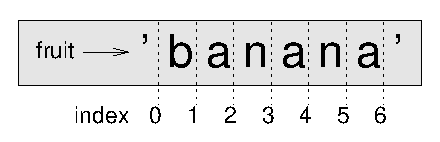
\includegraphics{figs/banana.eps}}
\afterfig

如果你忽略第一个下标(在冒号之前),切片开始于字符串的头部。如果你忽略第二个下标,切片将结束于字符串的尾部:

\beforeverb
\begin{verbatim}
>>> fruit = 'banana'
>>> fruit[:3]
'ban'
>>> fruit[3:]
'ana'
\end{verbatim}
\afterverb
%
如果第一个下标大于等于第二个下标,结果将为一个{\bf 空字符串},用两个引号表示:

\index{引号标记}

\beforeverb
\begin{verbatim}
>>> fruit = 'banana'
>>> fruit[3:3]
''
\end{verbatim}
\afterverb
%
空字符串不包含任何字符且长度为零,除此以外和其他字符串相同。

\begin{ex}
假设{\tt fruit}是一个字符串,{\tt fruit[:]}是什么?

\index{复制!切片}
\index{切片!复制}

\end{ex}


\section{字符串是不变的}
\index{可变}
\index{不可变}
\index{字符串!不可变}

下面尝试使用{\tt []}运算符作为赋值语句的左值,试图改变字符串中的字符:

\index{类型错误}
\index{异常!类型错误}

\beforeverb
\begin{verbatim}
>>> greeting = 'Hello, world!'
>>> greeting[0] = 'J'
TypeError: object does not support item assignment
\end{verbatim}
\afterverb
%
在本例中”对象“是字符串,”项目“是你试图赋值的字符。现在,一个”对象“等同于一个数值,以后我们会重新进行定义。一个”项目“是序列中的一个值。

\index{对象}
\index{项目赋值}
\index{赋值!项目}
\index{不可变}

错误的原因是因为字符串是{\bf 不可变的},即你不可以修改一个已经存在的字符串。你可以做的是新建一个字符串并在原来的基础上修改:

\beforeverb
\begin{verbatim}
>>> greeting = 'Hello, world!'
>>> new_greeting = 'J' + greeting[1:]
>>> print new_greeting
Jello, world!
\end{verbatim}
\afterverb
%
例子中将新的第一个字母和{\tt greeting}的一个切片连接,这个操作对原来字符串没有影响。

\index{连接}


\section{搜索}
\label{查找}

以下函数实现了什么功能?

\index{find函数}
\index{函数!find}

\beforeverb
\begin{verbatim}
def find(word, letter):
    index = 0
    while index < len(word):
        if word[index] == letter:
            return index
        index = index + 1
    return -1
\end{verbatim}
\afterverb
%
从某种角度来说,{\tt find}是{\tt []}运算符的反操作。它读取字符,寻找字符串中对应的下标。如果字符没有找到,函数返回{\tt -1}。

这是我们看到的第一个{\tt return}语句在循环体中的例子。如果{\tt word[index] == letter},函数中断跳出循环,并立即返回。

如果字符串中不存在该字符,程序正常退出循环并返回{\tt -1}。

这种遍历序列寻找我们需要的内容的计算模式称为{\bf 搜索}。

\index{遍历}
\index{搜索模式}
\index{模式!搜索}

\begin{ex}
修改{\tt find}函数,增加第三个参数{\tt word},指示开始搜索的位置。
\end{ex}


\section{循环和记数}
\label{记数}

\index{记数}
\index{记数和循环}
\index{循环和记数}
\index{循环!关于字符串}

下面的程序统计字符{\tt a}在字符串中出现的次数:

\beforeverb
\begin{verbatim}
word = 'banana'
count = 0
for letter in word:
    if letter == 'a':
        count = count + 1
print count
\end{verbatim}
\afterverb
%
程序演示了另一种计算模式{\bf 记数}。变量{\tt count}首先被初始化为0,然后每次发现{\tt a}就增加1。当循环退出后,{\tt count}记录了{\tt a}总共出现的次数。

\begin{ex}
\index{封装}

将代码封装成一个名叫{\tt count}的函数,推广函数是得它可以接收字符串和字符作为参数。

\end{ex}

\begin{ex}
重写函数,使用3个参数的{\tt find}版本,而不是遍历字符串。
\end{ex}


\section{{\tt string}方法}

{\bf 方法}类似函数,它读取参数,并返回一个值,但两者语法有区别。例如,方法{\tt upper}读取一个字符串并返回一个全大写的新字符串:

\index{方法}
\index{字符串!方法}

相比函数的语法{\tt upper(word)},方法的语法为{\tt word.upper()}。

\index{点符号}

\beforeverb
\begin{verbatim}
>>> word = 'banana'
>>> new_word = word.upper()
>>> print new_word
BANANA
\end{verbatim}
\afterverb
%
这样的点符号的形式指定了方法的名称{\tt upper},以及方法作用的字符串名{\tt word}。空的括号指示这个方法不读取参数。

\index{括号!空}

一个方法的调用称为{\bf 调用};在本例中,我们称对{\tt word}调用了{\tt upper}方法。

\index{调用}

事实上,字符串有一个方法{\tt find}十分类似我们写的函数:

\beforeverb
\begin{verbatim}
>>> word = 'banana'
>>> index = word.find('a')
>>> print index
1
\end{verbatim}
\afterverb
%
在这个例子中,我们对{\tt word}调用了{\tt find}方法,并传入我们需要寻找的字符作为参数。

事实上,{\tt find}方法比我们的函数适用更广,它不仅可以查找字符,也可以查找子串:

\beforeverb
\begin{verbatim}
>>> word.find('na')
2
\end{verbatim}
\afterverb
%
它可以读取第二个参数来指定开始查找的位置:

\index{可选参数}
\index{参数!可选}

\beforeverb
\begin{verbatim}
>>> word.find('na', 3)
4
\end{verbatim}
\afterverb
%
还有第三个参数,指定查找结束的位置:

\beforeverb
\begin{verbatim}
>>> name = 'bob'
>>> name.find('b', 1, 2)
-1
\end{verbatim}
\afterverb
%
这次查找失败,因为{\tt b}在查找范围{\tt 1}到{\tt 2}中不存在(不包含{\tt 2})。


\begin{ex}
\index{记数方法}
\index{方法!记数}

字符串有个方法称为{\tt count},类似先前练习中的函数。阅读这个方法的文档,编写方法调用,统计{\tt a}在\verb"'banana'"中出现的次数。
\end{ex}


\section{{\tt in}运算符}
\label{inboth}

\index{in运算符}
\index{运算符!in}
\index{布尔运算符}
\index{运算符!布尔}

{\tt in}是一个布尔运算符,它读取两个字符串作为参数,如果第一个字符串是第二个字符串的子串,则返回{\tt True}:

\beforeverb
\begin{verbatim}
>>> 'a' in 'banana'
True
>>> 'seed' in 'banana'
False
\end{verbatim}
\afterverb
%
例如,下面的函数打印在{\tt word1}和{\tt word2}中同时出现的字符:

\beforeverb
\begin{verbatim}
def in_both(word1, word2):
    for letter in word1:
        if letter in word2:
            print letter
\end{verbatim}
\afterverb
%
如果函数名是精心挑选的,Python有时读起来想英语。你可以这么读一个循环:“for (each) letter in (the first) word, if (the) letter (appears) in (the second) word, print (the) letter.”

下面是你比较apples和oranges的输出:

\beforeverb
\begin{verbatim}
>>> in_both('apples', 'oranges')
a
e
s
\end{verbatim}
\afterverb
%

\section{字符串比较}

\index{字符串!比较}
\index{比较!字符串}

关系运算符可以作用在字符串上。看两个字符串是否相等:

\beforeverb
\begin{verbatim}
if word == 'banana':
    print  'All right, bananas.'
\end{verbatim}
\afterverb
%
其他关系运算符可以用来将单词按字母表排序:

\beforeverb
\begin{verbatim}
if word < 'banana':
    print 'Your word,' + word + ', comes before banana.'
elif word > 'banana':
    print 'Your word,' + word + ', comes after banana.'
else:
    print 'All right, bananas.'
\end{verbatim}
\afterverb
%
Python不像人们一样处理大小写字母。所有的大写字母在小写字母之前,所以:

\beforeverb
\begin{verbatim}
Your word, Pineapple, comes before banana.
\end{verbatim}
\afterverb
%
一个常用的解决这个问题的方法是在比较前将字符串转化为一个标准的格式,如全小写。


\section{调试}
\index{调试}

\index{遍历}
当使用下标遍历序列的值时,很容易将遍历的开始位置和结束位置搞错。这里给出了一个函数,它试图比较两个单词,如果一个是另一个的逆序则返回{\tt True},函数中有两个错误:

\beforeverb
\begin{verbatim}
def is_reverse(word1, word2):
    if len(word1) != len(word2):
        return False
    
    i = 0
    j = len(word2)

    while j > 0:
        if word1[i] != word2[j]:
            return False
        i = i+1
        j = j-1

    return True
\end{verbatim}
\afterverb
%
第一个{\tt if}语句检查两个单词是否长度相同。如果不相同,我们可以立即返回{\tt False}。否则,我们可以保证两个单词长度相同。这是章节~\ref{守护人}中一个守护人模式的例子。

\index{守护人模式}
\index{模式!守护人}
\index{下标}

{\tt i}和{\tt j}是下标,{\tt i}从前往后遍历{\tt word1},而{\tt j}从后往前遍历{\tt word2}。如果我们发现两个字符不同,我们可以立即返回{\tt False}。如果我们完成整个循环,即所有字符都匹配,我们返回{\tt True}。

如果我们用“pots”和“stop”来测试这个函数,我们期望返回值为{\tt True},然而我们得到下标错误:

\index{下标错误}
\index{异常!下标错误}

\beforeverb
\begin{verbatim}
>>> is_reverse('pots', 'stop')
...
  File "reverse.py", line 15, in is_reverse
    if word1[i] != word2[j]:
IndexError: string index out of range
\end{verbatim}
\afterverb
%
为了调试这类错误,我第一步是在错误的行前面打印相应的值:

\beforeverb
\begin{verbatim}
    while j > 0:
        print i, j        # print here
        
        if word1[i] != word2[j]:
            return False
        i = i+1
        j = j-1
\end{verbatim}
\afterverb
%
现在再次运行程序,我得到更多的信息:

\beforeverb
\begin{verbatim}
>>> is_reverse('pots', 'stop')
0 4
...
IndexError: string index out of range
\end{verbatim}
\afterverb
%
在第一次穿越循环后,{\tt j}的值是4,超过了\verb"'pots'"的长度。最后一个字符对应的下标是3,所以{\tt j}的初始值应该为{\tt len(word2)-1}。

\index{语义错误}
\index{错误!语义}

我修正了这个错误,再次运行程序得到:

\beforeverb
\begin{verbatim}
>>> is_reverse('pots', 'stop')
0 3
1 2
2 1
True
\end{verbatim}
\afterverb
%
这次我们得到正确的结果,但看起来循环只运行了3次,十分可疑。为了弄清楚是怎么回事,一个很有效的方法是画状态图。在第一次迭代中,\verb"is_reverse"的第一帧如下:

\index{状态图}
\index{图!状态}

\beforefig
\centerline{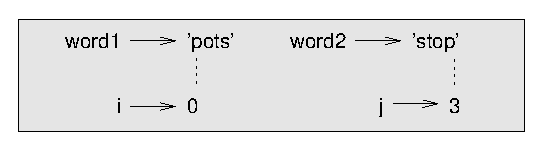
\includegraphics{figs/state4.eps}}
\afterfig

我用虚线标记出变量{\tt i}和{\tt j}对应{\tt word1}和{\tt word2}中的字符。

\begin{ex}
\label{is_reverse}
从这个图开始,在纸上运行程序,在每次迭代中修改{\tt i}和{\tt j}的值。找出并修改函数中的错误。
\end{ex}



\section{术语}

\begin{description}

\item[对象:] 变量可以指向的东西。到目前,你可以互换的使用“对象”和“值”。
\index{对象}

\item[序列:] 一个有序的集合,每一个集合中的数对应一个整数下标。
\index{序列}

\item[项目:] 序列中的一个项目。
\index{项目}

\item[下标:] 序列中用于选择项目的一个整数值,如字符串中的一个字符。
\index{下标}

\item[切片:] 有一定下标确定的字符串的一部分。
\index{切片}

\item[空字符串:] 一个没有字符的长度为0的字符串,使用两个引号表示。
\index{空字符串}

\item[不可变:] 序列中的项目不可改变的性质。
\index{不可变}

\item[遍历:] 迭代访问序列中的每个项目,并执行类似的操作。
\index{遍历}

\item[查找:] 遍历的一种模式,当找到要找的内容时停止。
\index{查找模式}
\index{模式!查找}

\item[计数器:] 用来计数的变量,通常初始化为0,然后递增。
\index{计数器}

\item[方法:] 一个和对象关联的函数,应用点符号来调用。
\index{方法}

\item[调用:] 调用方法的语句。
\index{调用}

\end{description}


\section{练习}

\begin{ex}

\index{步长}
\index{切片运算符}
\index{运算符!切片}

字符串的切片可以读取第三个参数“步长”,它决定了相邻字符之间的间隔。步长为2意味着每隔一个字符,步长为3意味着隔两个字符,以此类推。

\beforeverb
\begin{verbatim}
>>> fruit = 'banana'
>>> fruit[0:5:2]
'bnn'
\end{verbatim}
\afterverb

步长为-1对应从后往前遍历单词,因此\verb"[::-1]"将产生一个翻转的字符串。

\index{回文}

使用这个写法编写一个一行版本的\verb"is_palindrome"函数,类似练习~\ref{回文}。
\end{ex}


\begin{ex}
\index{字符串方法}
\index{方法!字符串}

阅读字符串的方法\url{docs.python.org/lib/string-methods.html}。你需要使用部分函数来确保你理解它们是如何工作的。{\tt strip}和{\tt replace}特别有用。

文档使用的语法可能令人困惑。比如,在\verb"find(sub[, start[, end]])"中,括号表示参数是可选的。因此{\tt sub}是必须的,而{\tt start}是可选的,如果你包含了{\tt start},那么{\tt end}是可选的。
\end{ex}

\begin{ex}
下面的函数都{\em 试图}检查一个字符串是否包含小写字母,但至少它们中的一些是错误的。对于每个函数,描述它们实际上做了什么(假设参数是一个字符串)。

\beforeverb
\begin{verbatim}
def any_lowercase1(s):
    for c in s:
        if c.islower():
            return True
        else:
            return False

def any_lowercase2(s):
    for c in s:
        if 'c'.islower():
            return 'True'
        else:
            return 'False'

def any_lowercase3(s):
    for c in s:
        flag = c.islower()
    return flag

def any_lowercase4(s):
    flag = False
    for c in s:
        flag = flag or c.islower()
    return flag

def any_lowercase5(s):
    for c in s:
        if not c.islower():
            return False
    return True
\end{verbatim}
\afterverb

\end{ex}


\begin{ex}
\index{字符旋转}
\index{旋转,字符}

\label{exrotate}
ROT13是一种弱的加密方式,它将单词中的每个字母“旋转”13个单位\footnote{参见 \url{wikipedia.org/wiki/ROT13}。}。旋转一个字母意味着按字母顺序移动,有必要时绕回开始的位置,因此'A'移动3个单位是'D','Z'移动1个单位是'A'。

编写函数\verb"rotate_word",读取一个字符串和一个整数作为参数,返回一个新的字符串,它是在原来的字符串的字符“旋转”给定的量。

比如,“cheer”旋转7个单位是“jolly”,“melon”旋转-10个单位是“cubed”。

%For example ``sleep''
%rotated by 9 is ``bunny'' and ``latex'' rotated by 7 is ``shale''.

你也许会用到内建函数{\tt ord},它将字符转换为一个数字代码,以及函数{\tt chr},将数字代码转换为一个字符。

网上一些攻击性的玩笑有时候使用ROT13来加密的,如果你不是轻易被冒犯的,寻找并解码它们。
\end{ex}




\chapter{实例学习:字符处理}

\section{读取单词表}
\label{wordlist}

我们本章的联系需要一个英语单词表。在网络上有数以万计的单词表,但是
最适合我们的一个是贡献给公共域的单词表,它是由Grady Ward搜集整理作为Moby词典工程的一部分\footnote{\url{wikipedia.org/wiki/Moby_Project}.}。
它由113,809个官方纵横组合字谜的单词组成,也就是在纵横组合字谜中和其他字谜游戏中存在的单词组成。在Moby的搜集中,文件名是{\tt 113089.fic};我
复制了这个文件,命名为{\tt words.txt},并把它包含在了Swampy里了。

\index{Swampy}
\index{crosswords 纵横组合字谜}


这个文件是纯文本文件,你可以用一个编辑器打开它,当然,你也可以用python
来读取它。内置函数{\tt open}接受一个文件名作为参数,返回一个文件对象,
用它可以读取文件。

\index{oepn function open函数}
\index{function!open}
\index{plain text 纯文本文件}
\index{text!plain}
\index{object!file}
\index{file object  文件对象}

\beforeverb
\begin{verbatim}
>>> fin = open('words.txt')
>>> print fin
<open file 'words.txt', mode 'r' at 0xb7f4b380>
\end{verbatim}
\afterverb

{\tt fin}是赋给用来输入的文件对象的常见名称。大开模式\verb"'r'"表明
文件以只读方式大开(和\verb"'w'"以只写模式打开相反)。

\index{redline method readline方法}
\index{methods!readline}

文件对象提供了多种方式来读取文件,其中就包括{\tt readline},该函数从
文件中读取字符知道遇到换行符,然后以字符串的形式返回结果:

\beforeverb
\begin{verbatim}
>>> fin.readline()
'aa\r\n'
\end{verbatim}
\afterverb
%

这个单词表的第一个单词是"aa,"是一种熔岩的名称。序列\verb"\r\n"代表两个
空白字符,回车和换行,它们把这个单词下一行分隔开来。

文件对象自己跟踪达到了文件的什么地方,所以当再次调用{\tt readline}函数时,就会得到下一个单词:

\beforeverb
\begin{verbatim}
>>> fin.readline()
'aah\r\n'
\end{verbatim}
\afterverb

下一个单词是"aah,"---绝对合法的一个单词,不要以那么怪的眼神看我\footnote{译者:我没有笑话你的意思哦}。如果那个whitespace看上去很不给力,我们
使用{\tt strip}函数剔除它:

\index{strip method strip方法}
\index{method!strip}

\beforeverb
\begin{verbatim}
>>> line = fin.readline()
>>> word = line.strip()
>>> print word
aahed
\end{verbatim}
\afterverb

也可以在{\tt for}循环中使用文件对象。下面的程序对去{\tt word.txt},打印每一个单词,一行一个:

\index{open function open函数}
\index{function!open}

\beforeverb
\begin{verbatim}
fin = open('words.txt')
for line in fin:
    word = line.strip()
    print word
\end{verbatim}
\afterverb

\begin{ex}
编写一个程序,读取{\tt words.txt},打印包含超过20个字符的单词(不包括空白)。

\index{whitespace 空格}

\end{ex}

\section{练习}

下个部分有这些练习的答案。你至少得在参看答案之前尝试做一做每一道题。

\begin{ex}

1939年,Ernest Vincent Wright发表了一本50,000字的小说{\em Gadsby},在这本书中
不包含字母“e“。"e"在英语中是非常常见的字母,所以这件事很难做到。

事实上,如果不使用最常见的符号是很难想象那样的情况的。开始进展比较缓慢,但是
谨慎地训练几个小时之后,你就会逐步的掌握要领。

好的,进入正题!

编写一个函数\verb"has_no_e",如果给定的单词不含有字母"e",返回{\tt True}。

修改上一部分的程序,打印不含有"e"的单词,并计算不含有"e"的单词的百分比。

\index{lipogram 避讳}

\end{ex}

\begin{ex}

编写一个函数{\tt avoids}接受一个单词和一串“禁止”字母,如果单词没有使用禁止
字母中的任何一个,返回{\tt True}

修改你的程序提示用户输入一串禁止字母,然后打印不含有它们中任意一个的单词数目。你能找出由5个“禁止”字母组成的单词,不包括最小数目的单词吗?

\end{ex}

\begin{ex}
编写一个函数\verb"uses_only",接受一个单词和一串字母,如果单词仅仅包含列表
字符串里的字母,返回{\tt True}。除了"Hoe alfalfa"你能用{\tt acefhlo}里的字母
造一个句子吗?
\end{ex}

\begin{ex}

编写一个函数\verb"uses_all",接受一个单词和一串字母,如果单词使用一串字母里
的所有字母(至少一次),返回{\tt True}。有多少单词包含了全部的元音{\tt aeiou}?{\tt aeiouy}呢?
\end{ex}


\begin{ex}
编写一个函数\verb"is_abecedarian",如果单词里的字母以字典顺序出现,返回{\tt True}。有多少{\tt abecedarian}式的单词?
\end{ex}

\index{abecedarian}

\section{搜索}

\index{search pattern 搜索模式}
\index{pattern!search}






前一部分的所有联系都有一个共同点:他们都可以通过一个可搜索模式来解决,我们
在\ref{find}部分遇到过。最简单的例子是:

\beforeverb
\begin{verbatim}
def has_no_e(word):
    for letter in word:
        if letter == 'e':
            return False
    return True
\end{verbatim}
\afterverb

{\tt for}循环遍历{\tt word}中的每一个字母;如果不匹配,就进入下一个字母。
如果我们正常退出循环,就意味着我们没有找到“e“,于是返回{\tt True}。

\index{traversal 遍历}

\index{generalization}

{\tt avoids}是一个更一般的\verb"has_no_e"版本,但是有着相同的结构:

\beforeverb
\begin{verbatim}
def avoids(word, forbidden):
    for letter in word:
        if letter in forbidden:
            return False
    return True
\end{verbatim}
\afterverb

如果发现一个“禁止”字母,我们就返回{\tt False};如果我们达到了循环的结尾,
就返回{\tt True}。

\verb"uses_only"和它类似,出了条件的意思是相反的。

\beforeverb
\begin{verbatim}
def uses_only(word, available):
    for letter in word: 
        if letter not in available:
            return False
    return True
\end{verbatim}
\afterverb

除了使用一串“禁止”字母,我们也可以使用可获得字母(avaliable)。如果我们在、
{\tt word}中发现一个字母不再可获得字母中,就返回{\tt False}。

\verb"uses_all"函数也类似,出了我们掉换了word 和一串字母的角色。
\beforeverb
\begin{verbatim}
def uses_all(word, required):
    for letter in required: 
        if letter not in word:
            return False
    return True
\end{verbatim}
\afterverb

我们没有遍历{\tt word}中的字母,循环遍历了“要求“的字母,如果任意一个“要求”
字母没有出现在{\tt word}中,我们返回{\tt False}。

\index{traversal 遍历}

如果你想像一个计算机科学家一样思考,你可能已经认出\verb"uses_all"是前面已经
解决过的问题的实例,你就会编写:

\beforeverb
\begin{verbatim}
def uses_all(word, required):
    return uses_only(required, word)
\end{verbatim}
\afterverb

这是程序设计方法中的一个实例---叫做问题识别,含义是你认识到现在解决的问题
是已经解决问题的一个实例,然后修改应用以前的解法。

\index{problem recognition 问题识别}
\index{development plan!problem recognition}

\section{使用索引循环}

\index{looping!with indices}
\index{index!looping with}

我用{\tt for}循环编写以前的函数,因为我只需要用到字符串里的字符;我没有必要
使用索引来解决问题。

对于\verb"is_abecedarian"我们必须要比较相邻的字母,{\tt for}循环就有点力不
从心了。




\beforeverb
\begin{verbatim}
def is_abecedarian(word):
    previous = word[0]
    for c in word:
        if c < previous:
            return False
        previous = c
    return True
\end{verbatim}
\afterverb

另外一种方法就是使用递归:

\beforeverb
\begin{verbatim}
def is_abecedarian(word):
    if len(word) <= 1:
        return True
    if word[0] > word[1]:
        return False
    return is_abecedarian(word[1:])
\end{verbatim}
\afterverb

也还可以使用{\tt while}循环:

\beforeverb
\begin{verbatim}
def is_abecedarian(word):
    i = 0
    while i < len(word)-1:
        if word[i+1] < word[i]:
            return False
        i = i+1
    return True
\end{verbatim}
\afterverb


循环从{\tt i = 0}开始,以{\tt i = len(word) -1}收尾。每次循环时,比较第$i$
(你可以把它当成当前的字符)和$i+1$字符(你可以把它当作第二个字符)。

如果下一个字符小于当前的字符(字典顺序是在前),字母次序就被打断了,我们
返回{\tt False}。

如果我们到达了循环的末尾并且没有发现错误,这个{\tt word}“通过“了测试。
为了让自己信服循环正确的结束了,考虑这样一个例子\verb"'flossy'"。这个单词
的长度是6,所以最后一次循环执行的时候{\tt i} 是4---正好是倒数第二个字符的索引。
在最后一次迭代中,程序比较倒数第二个字符和最后一个字符---这就是我们希望的~。

\index{palindrome 回文}

下面是一个\verb"is_palindrome"的版本(参看练习\ref{回文}) ,函数使用了两个
索引;一个从头部开始,逐步递增,另外一个从尾部开始,逐步递减。


\beforeverb
\begin{verbatim}
def is_palindrome(word):
    i = 0
    j = len(word)-1

    while i<j:
        if word[i] != word[j]:
            return False
        i = i+1
        j = j-1

    return True
\end{verbatim}
\afterverb

或者,你也注意到了这又是已解决问题的一个实例,你或许会这么写:

\beforeverb
\begin{verbatim}
def is_palindrome(word):
    return is_reverse(word, word)
\end{verbatim}
\afterverb

\index{problem recognition 问题识别}
\index{development plan!problem recognition}

我认为你做了练习\ref{is_reverse}。

\section{调试}

\index{debugging 调试}
\index{testing!is hard}
\index{program testing 程序测试}

测试程序是一种“折磨”。本章的函数相对来说比较容易测试,因为你可以手动的检查
输出结果。尽管如此,某些地方还是很难甚至不可能选择一个合适的单词表来测试
所有可能的错误。\\


拿\verb"has_no_e"做例子,有两种明显的情况需要测试:含有"e"的单词应该返回{\tt False};不含有的返回{\tt True}。对于这两种情况,应该都没有任何错误。\\


在这两中情况下又有一些不太明显的子情况。在含有“e“的单词中,我们应该测试
"e"在单词前,在单词尾,在中间的某个地方。也应该测试长单词,短单词,和非常
短的单词,像空字符串。空字符串是特殊情况中的一个例子,也是非常不明显的情况,而错误恰恰经常藏身此处。

\index{special case 特别情况}

除了测试你自己想出的情况,你也可以用单词表来测试,比如使用{\tt word.txt}。
通过查看输出,你就可以抓住错误,但是小心:你或许能抓住一种错误(本不该包括
的单词被包括了)但不是另外一种(本该包含的单词没有被包含)。

一般说来,测试能帮助我们发现bugs,但是产生好的测试案例不是一件容易的事,
而且即使你测试了,你也不能保证你的程序就是正确的。

\index{testing!and absence of bugs}

一位传奇式的计算机科学家这么说过:

\begin{quote}
程序测试能够发现bugs是存在的,但是永远发现不了bugs不存在。

---Edsger W.Dijkstra
\end{quote}

\index{Dijkstra, Edsger}

\section{术语表}

\begin{description}

\item [file object 文件对象:] 代表打开文件的数值。
\index{file object 文件对象}
\index{object!file}

\item [problem recognition 问题识别:]通过把问题阐释成已经解决问题的一个
实例来解决问题的方法。
\index{problem recognition 问题识别}

\item [special case 特殊情况:]非典型的或不明显的测试例子(很难完美解决)。
\index{special case 特殊情况}

\end{description}

\section{练习}

\begin{ex}


\index{Car Talk 汽车谈话}
\index{Puzzler 难题}
\index{double letters }

这个问题是基于广播节目{\em Car Talk}播发的一个难题\footnote{\url{www.cartalk.com/content/puzzler/transcripts/200725}.}:

\begin{quote}

 给我一个含有三个连续的双字母单词,我能给你几个几乎符合条件的单词,但是不是
 完全符合。比如,单词{\tt committee},c-o-m-m-i-t-t-e-e。如果没有了$i$在那里,会更完美;Mississippi也是:M-i-s-s-i-s-s-i-p-p-i。如果能够去掉这些$i$,
 结果就很完美。有一个单词有三个连续的双字母,据我所知,只有这一个。当然,
 也有可能有500多个,但是我只能想到这一个。那么这个单词是什么?
 \end{quote}

 编写一个程序,寻找它。你可以参看我的答案\url{thinkpython.com/code/cartalk.py}.

\end{ex}



\begin{ex}
下面的也是一个{\em Car Talk}难题\footnote{\url{www.cartalk.com/content/puzzler/transcripts/200803}.}:

\index{Car Talk}
\index{Puzzler 难题}
\index{odometer 里程表}
\index{palindrome 回文}


\begin{quote}
“有一天,我驾车在高速公路上行使,我偶然看到了我的里程表。像大多数的里程表
一样,它显示了六个数字,全部是里数。比如,如果我的小汽车行使额300,000里,
我将会看到3-0-0-0-0-0。\\

“现在,我那天看到的却是非常的有意思。我注意到后四个数字是回文的;也就是说
从前往后读和从后往前读是一样的。比如,5-4-4-5是回文,所以我的里程表可能显示3-1-5-4-4-5。\\

“行使了一里之后,后五位数是回文的了。比如,可能是3-6-5-4-5-6。再行使一里后
中间的四位又是回文的了。你或许猜到了,一公里后,六位数字是回文的了!\\

“问题是,当我第一次看里程表的时候,显示的是什么?”
\end{quote}

编写一个Python程序,测试所有的六位数,打印任何满足条件的数字。你可以参看我的答案\url{thinkpython.com/code/cartalk.py}.

\end{ex}

\begin{ex}

下面的又是一个{\em Car Talk}难题,你可以用搜索来解决它\footnote{\url{www.cartalk.com/content/puzzler/transcripts/200813}}:

\index{Car Talk}
\index{Puzzler  难题}
\index{palindrome 回文}

\begin{quote}
“最近,我拜访了妈妈。我们认识到组成我年龄的两位数倒过来时是她的年龄。
比如,如果她是73,我就是37。我们想知道这种事发生的频率是多少?但是我们
转移到了另外一个话题,我们也就没有得到答案。\\

“当我会到家的时候,我计算出组成我们年龄的两位数已经有六次是像上面那样
了。我也计算出,如果幸运的话,几年后又会发生了,如果我们真的幸运的话,
在那之后,还会一次。也就是说,总共会有8次。现在的问题是,我今年多大了?”

\end{quote}

编写一个Python程序,搜索这个难题的答案。Hint:你或许会发现字符串方法{\tt zfill}对你有些帮助。

可以参看我的答案\url{thinkpython.com/code/cartalk.py}.

\end{ex}






























\chapter{列表}


\chapter{字典}


\chapter{元组}


\chapter{实例学习:数据结构的实例}


\chapter{文件}


\chapter{类和对象}


\chapter{类和函数}


\chapter{类和方法}


\chapter{继承}


\chapter{实例学习:Tkinter}

\section{GUI}

我们迄今为止编写的程序都是字符界面下的,现在很多程序使用
图形用户接口(graphical user interfaces},简称{\bf GUIs}。

\index{GUI}
\index{graphical user interface 图形用户接口}
\index{Tkinter}

Python提供了多种选择来来编写GUI程序,包括wxPython, Tkinter和
Qt\footnote{译注:还有一个非常流行的就是pyGtk}。每种框架都优缺参半。
这也就是为什么Python在图形库上没有形成一个标准的原因。

这一章,我要讲述的是Tkinter,因为我认为它是最容易入手的。本章的很多概念同样适用于其他GUI模块。

有一些关于Tkinter的书和网站。网上最好的资料是Fredrik Lundh写的{\em An Introduction to Tkinter}。

\index{Gui module}
\index{module!Gui}
\index{Swampy}

我也写了一个模块{\tt Gui.py},包含在Swampy里。它提供了Tkinter里函数和
类的简单接口。这章的例子就是以这个模块为基础。

下面是一个创建显示Gui的简单例子:

要创建一个GUI,必须导入{\tt Gui}模块,并且实例化一个Gui对象:

\beforeverb
\begin{verbatim}
from Gui import *

g = Gui()
g.title('Gui')
g.mainloop()
\end{verbatim}
\afterverb
%

当运行这段代码,会出现一个窗口,窗口由灰色的区域和标题{\sf Gui}组成。
{\tt mainloop}运行事件循环,等待用户操作,然后做出相应的反应。这是一个无限循环,一直运行到用户关闭窗口,或者按下Control-C,或者其他能使程序终止的操作。

\index{event loop 事件循环}
\index{loop!event}
\index{infinite loop 无限循环}
\index{loop!infinite}

这个Gui没有做什么事情,因为它没有任何的控件。控件是构成GUI的元素,
包括:

\index{widget 控件}

\begin{description}

\item [Button 按钮:]包含文本或图像的控件,当被按压时,产生一个动作。

\item [Canvas 画布:]能够显示直线,矩形,圆和其他图形的区域。

\item [Entry 输入框:]用户可以输入文本的区域。

\item [Scrollbar 滚动条:] 控制其他空间可见部分的空间。

\item [Frame 框:]容纳其他控件的容器,通常是不可见的。

\end{description}

创建Gui时的空白灰色区域就是一个框。当新建一个控件,就会被加到这个框。

\section{按钮和回调}

\index{Button widget 按钮控件}
\index{widget!Button}

{\tt bu}方法创建一个按钮空间:

\beforeverb
\begin{verbatim}
button = g.bu(text='Press me.')
\end{verbatim}
\afterverb

{\tt bu}方法的返回值是按钮对象。框里的按钮是这个对象的图形化显示;
可以通过调用按钮的方法控制按钮。

\index{option}

{\tt bu}可以通过32个参数控制按钮的外形和功能,这些参数叫做选项。除了
提供全部的32个选项,你可以提供关键的参数,像\verb"text='Press me.'",
指定你需要的选项即可,其他的使用缺省值。

\index{keyword argument 关键参数}
\index{argument!keyword}

当向一个框添加控件时,框就变被”收缩包裹“了,也就是框收缩成按钮般大小。
如果想添加更多的空间,框自动增长来安排他们。

\index{Label widget}
\index{widget!Label}

{\tt la}方法创建标签控件:

\beforeverb
\begin{verbatim}
label = g.la(text='Press the button.')
\end{verbatim}
\afterverb

缺省情况下,Tkinter从上至下安排空间,然后使其居中。我们不久将会看到如何覆盖这种行为。

如果按下按钮,你会看到它也没有做什么事情。那是因为你还没有“启动”它,也就是说,你还没有告诉它做什么!

控制一个按钮行为的选项是{\tt command}。{\tt command}的值是一个函数,它在按钮按下的时候执行。比如,下面是一个函数创建一个新的标签:

\beforeverb
\begin{verbatim}
def make_label():
    g.la(text='Thank you.')
\end{verbatim}
\afterverb

现在我们可以创建一个按钮,把这个函数作为{\tt command}:

\beforeverb
\begin{verbatim}
button2 = g.bu(text='No, press me!', command=make_label)
\end{verbatim}
\afterverb

当按下这个按钮,程序执行\verb"make_label",一个新的标签就会出现。

\index{callback 回调}

{\tt command}的值是一个函数对象,也叫回调函数,因为当你调用{\tt bu}
创建一个按钮,用户按下按钮时,执行流回调了。

\index{event-driven programming 时间驱动编程}

这种控制流是事件驱动编程的特点。用户动作,像按下按钮和击键,叫做事件
。在事件驱动编程中,执行流是由用户动作控制而不是程序员。

事件驱动编程的最大挑战在于为任何的用户动作建立一系列的控件及回调函数(至少更产生适当的错误信息)。

\begin{ex}
编写一个程序,创建只有一个按钮的GUI。当按钮被按下时,程序创建第二个按钮。当第二个按钮被按下时,应该创建一个标签,显示"Nice job!"。

如果按了多次按钮,会出现什么情况?

可以参看我的解答\url{thinkpython.com/code/button_demo.py}

\end{ex}


\section{画布控件}

\index{Canvas widget 画布控件}
\index{widget!Canvas}

画布是用途最多的空间之一,创建一个可以绘制直线,圆,和其他形状的区域。如果你做了练习\ref{画布},你已经熟悉了画布。

{\tt ca}创建了一个新的画布:

\beforeverb
\begin{verbatim}
canvas = g.ca(width=500, height=500)
\end{verbatim}
\afterverb

{\tt width}和{\tt height}是用像素表示的画布尺度。

\index{config method}
\index{method!config}

在创建了一个控件之后,仍然可以通过{\tt config}方法来修改选项的值。比如,{\tt bg}选项改变背景颜色:

\beforeverb
\begin{verbatim}
canvas.config(bg='white')
\end{verbatim}
\afterverb

{\tt bg}的值是颜色名。不同的Python拥有不同的合法颜色名,但是所有的
python实现都会提供至少如下的颜色名:

\begin{verbatim}
white   black
red     green    blue   
cyan    yellow   magenta
\end{verbatim}
\afterverb
%

画布上的图形叫做项。比如,画布方法{\tt circle}绘制(你猜是这样)一个圆:

\index{Canvas item 画布项}
\index{item!Canvas}

\beforeverb
\begin{verbatim}
item = canvas.circle([0,0], 100, fill='red')
\end{verbatim}
\afterverb


第一个参数是一个坐标对,指明了圆心的位置;第二个是半径。

\index{Canvas coordinate 画布坐标}
\index{coordinate!Canvas}

{\tt Gui.py}提供了一个标准的笛卡尔坐标系,原点在画布的中央,$y$正
半轴向上。这个其他的图像系统不一样,他们的原点在左上角,$y$正半轴向下。

{\tt fill}选项指明圆应该用红色来填充。

{\tt circle}的返回值是一个项对象,提供了修改画布上项的方法。蔽日,
可以使用{\tt config}改变圆的任意一个选项:

\beforeverb
\begin{verbatim}
item.config(fill='yellow', outline='orange', width=10)
\end{verbatim}
\afterverb

{\tt width}是用像素表示的轮廓厚度;{\tt outline}是颜色。

\begin{ex}
\label{circle}

编写一个程序创建一个画布和按钮。当用户按下按钮,应该在华布上画一个圆。
\end{ex}

\section{坐标序列}

\index{coordinate sequence 坐标序列}
\index{sequence!coordinate}

{\tt rectangle}方法接受坐标序列指明对顶角的位置。下面这个例子
绘制了一个绿色的矩形,坐下角在原点,右上角在$(200,100)$:

\beforeverb
\begin{verbatim}
canvas.rectangle([[0, 0], [200, 100]], 
                 fill='blue', outline='orange', width=10)
\end{verbatim}
\afterverb

这种指定角的方法叫做界定盒子,因为,两个点界定了一个矩形。

\index{bouding box}

{\tt oval}接受一个界定的盒子,在矩形里绘制一个椭圆。

\beforeverb
\begin{verbatim}
canvas.oval([[0, 0], [200, 100]], outline='orange', width=10)
\end{verbatim}
\afterverb

{\tt line}接受坐标序列,绘制线段连接各个点。下面这个例子绘制了三角形的两个边:

\beforeverb
\begin{verbatim}
canvas.line([[0, 100], [100, 200], [200, 100]], width=10)
\end{verbatim}
\afterverb

{\tt polygon}接受同样的参数,但是它绘制了最后一条边(如果有必要),并且
填充它:

\beforeverb
\begin{verbatim}
canvas.polygon([[0, 100], [100, 200], [200, 100]],
               fill='red', outline='orange', width=10)
\end{verbatim}
\afterverb

\section{更多的控件}

\index{Text widget 文本空间}
\index{widget!Text}

Tkinter提供了两个控件让用户输入文本:一个输入框,只能单行输入,和
文本控件,可以输入多行。

\index{Entry widget 输入框}
\index{widget!Entry}

{\tt en}创建一个输入框:

\beforeverb
\begin{verbatim}
entry = g.en(text='Default text.')
\end{verbatim}
\afterverb

{\tt text}选项允许你在输入框创建时把文本放进输入框。{\tt get}方法
返回文本框的内容(可能被用户改变了):

\beforeverb
\begin{verbatim}
>>> entry.get()
'Default text.'
\end{verbatim}
\afterverb

{\tt te}创建一个文本控件:

\beforeverb
\begin{verbatim}
text = g.te(width=100, height=5)
\end{verbatim}
\afterverb
%

{\tt width}和{\tt height}是空间中字符数和行数的大小。

{\tt insert}把文本插入文本控件:

\beforeverb
\begin{verbatim}
text.insert(END, 'A line of text.')
\end{verbatim}
\afterverb
%

{\tt END}是一个特别的索引,代表文本框里的最后一个字符。

你可以指定用点索引(dotted index来插入字符,像{\tt 1.1},小数点前面
的数字代表行数,后面的代表列数。下面的例子把\verb"'nother'"加到第一行第一个字符之后。

\beforeverb
\begin{verbatim}
>>> text.insert(1.1, 'nother')
\end{verbatim}
\afterverb

{\tt get}方法从文本控件读取文本;接受起始索引作为参数。下面的例子返回文本控件的所有内容,包括换行符:

\beforeverb
\begin{verbatim}
>>> text.get(0.0, END)
'Another line of text.\n'
\end{verbatim}
\afterverb
%

{\tt delete}方法从文本控件里移除文本;下面的例子删除除了开头的两个字符:

\beforeverb
\begin{verbatim}
>>> text.delete(1.2, END)
>>> text.get(0.0, END)
'An\n'
\end{verbatim}
\afterverb
%

\begin{ex}
\label{circle2}

修改练习\ref{circle}的解答,增加一个输入框和按钮。当用户按下新增加的
按钮时,程序从输入框读取一个颜色名,用它改变圆的填充色。用{\tt config}修改圆,不要新建一个圆。

你的程序应该能处理没有无颜色名或者颜色名不合法的情况。

参看我的解答\url{thinkpython.com/code/circle_demo.py}.

\end{ex}

\section{排列控件}

迄今,我们只是上下安排控件,但是大多数的GUIs的布局都是很复杂的。比如,下面是一个稍微有点复杂的TurtleWorld(参看\ref{turtlechap}章节)。

\beforefig
\centerline{
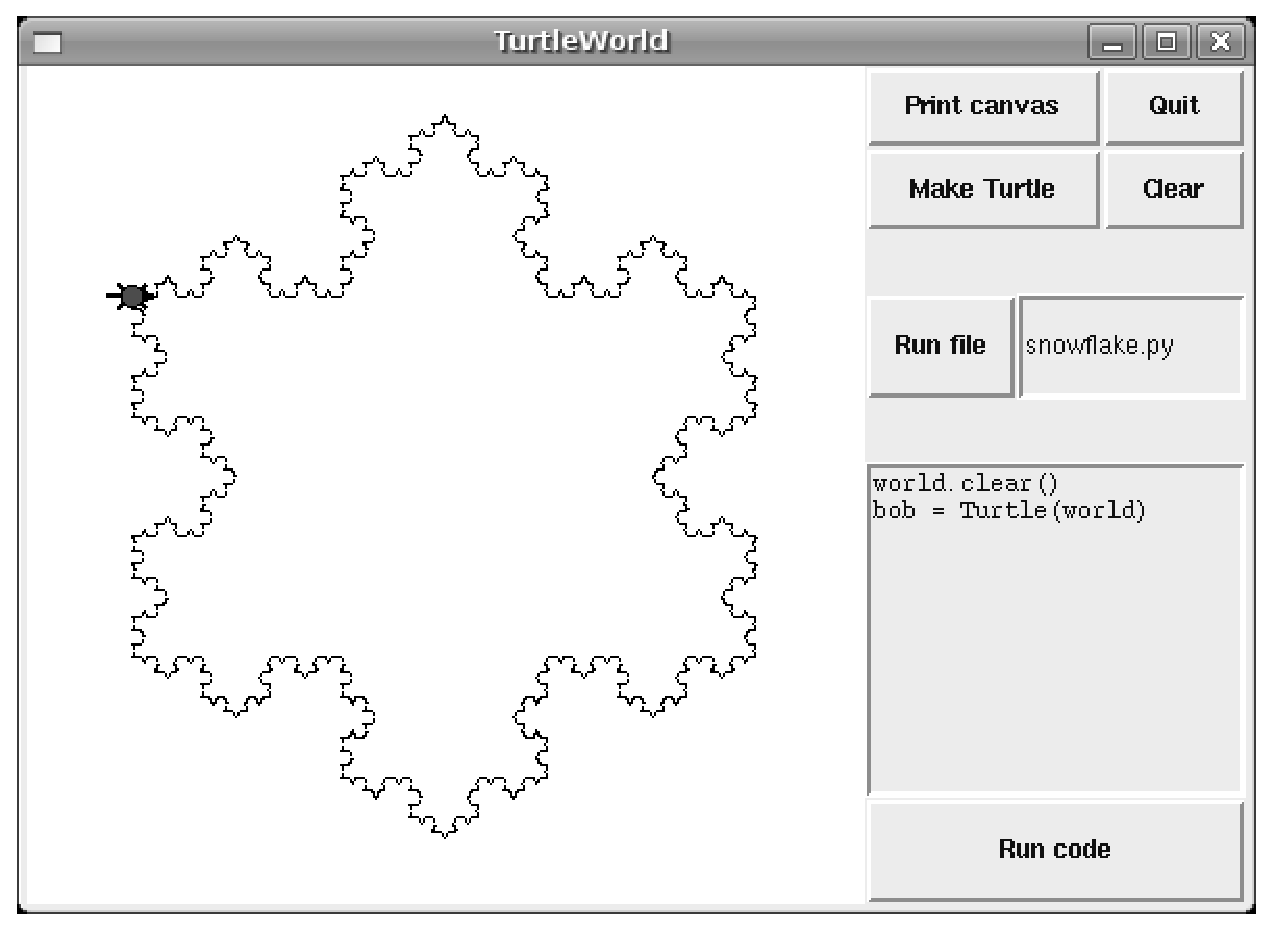
\includegraphics[width=1.0\textwidth]{figs/TurtleWorld.eps}
}
\afterfig


这个部分给出了创建这个GUI的代码,分解成一系列的步骤。可以下载完整的程序 \url{thinkpython.com/code/SimpleTurtleWorld.py}。

在顶级,这个GUI包含了两个控件---一个画布和一个框---并行排列着。所以第一步是创建行。

\index{SimpleTurtleWorld class}
\index{class!SimpleTurtleWorld}

\beforeverb
\begin{verbatim}
class SimpleTurtleWorld(TurtleWorld):
    """This class is identical to TurtleWorld, but the code that
    lays out the GUI is simplified for explanatory purposes."""

    def setup(self):
        self.row()
        ...
\end{verbatim}
\afterverb
%

{\tt setup}是创建并布局控件的函数。布局控件叫做包装。

\index{packing widgets 包装控件}
\index{widget,packing}
\index{Frame widget}
\index{widget!Frame}

{\tt row}行创建了一个行框,使它成为当前框。知道这个框被关闭或者新的框被船舰,所有后创建的控件都被包装在这行里。

下面是创建画布和列框,容纳其他控件的代码:

\beforeverb
\begin{verbatim}
        self.canvas = self.ca(width=400, height=400, bg='white')
        self.col()
\end{verbatim}
\afterverb
%

列框里的第一个控件是格子框,它包含了四个两两相邻的按钮。

\beforeverb
\begin{verbatim}
        self.gr(cols=2)
        self.bu(text='Print canvas', command=self.canvas.dump)
        self.bu(text='Quit', command=self.quit)
        self.bu(text='Make Turtle', command=self.make_turtle)
        self.bu(text='Clear', command=self.clear)
        self.endgr()
\end{verbatim}
\afterverb
%

{\tt gr}创建网格;参数是列的数目。网格里的控件是按照从左至右,从上到下安排的。

\index{callback 回调}
\index{bound method  绑定方法}
\index{method, bound}
\index{subject 主体}

第一个按钮使用{\tt self.canvas.dump}作为回调函数;第二个使用{\tt self.quit}。有三种绑定方法(bound methods),意味着他们和一个特定的对象绑定在一起。当他们被调用,他们是作用在该对象上。

列的下一个控件是行框,包含了一个按钮和输入框。

\beforeverb
\begin{verbatim}
        self.row([0,1], pady=30)
        self.bu(text='Run file', command=self.run_file)
        self.en_file = self.en(text='snowflake.py', width=5)
        self.endrow()
\end{verbatim}
\afterverb

{\tt row}的第一个参数是引力列表,决定了控件之间多余的空间如何分配。
{\tt [0,1]}表明所有的空间都分配给第二个控件,这里是输入框。如果你
运行这段代码,改变窗口大小,将会看到输入框变大而按钮不变。

选项{\tt pady}在$y$轴方向填充,上下分别增加30像素的空间。

{\tt endrow}结束添加控件,所以以后创建的可空间会被包装在列框。{\tt Gui.py}保存了框的栈:

\begin{itemize}

\item 当使用{\tt row},{\tt col},或者{\tt gr}创建一个框,程序进入栈顶,并且变为当前框。

\item 当使用{\tt endrow},{\tt endcol}或{\tt endgr}来关闭一个框,程序弹出栈顶,把前一个框置为当前框。

\end{itemize}

\verb"run_file"方法读取输入框的内容,把它作为文件名,读取文件,
传递给\verb"run_code"。{\tt self.inter}是一个解释器对象,能够接受一个字符串,并且把它作为Python代码执行。

\beforeverb
\begin{verbatim}
    def run_file(self):
        filename = self.en_file.get()
        fp = open(filename)
        source = fp.read()
        self.inter.run_code(source, filename)
\end{verbatim}
\afterverb
%

最后两个控件是文本控件和按钮:

\beforeverb
\begin{verbatim}
        self.te_code = self.te(width=25, height=10)
        self.te_code.insert(END, 'world.clear()\n')
        self.te_code.insert(END, 'bob = Turtle(world)\n')

        self.bu(text='Run code', command=self.run_text)
\end{verbatim}
\afterverb
%

\verb"run_text"和\verb"run_file"相似,除了它从文本控件接受代码,
而不是从文件:

\beforeverb
\begin{verbatim}
    def run_text(self):
        source = self.te_code.get(1.0, END)
        self.inter.run_code(source, '<user-provided code>')
\end{verbatim}
\afterverb

不幸的是,控件布局的方式和其他语言是有差异的,甚至在Python的不同模块里也是有差异的。Tkinter自己也提供了3种不同的布局控件的方式。这些方法叫做几何管理器。这部分我演示的是“grid"几何管理器;其他的两种叫做"组装“和”放置“。

\index{geometry manager 几何管理器}

幸运的是,这部分的大多数概念对其他的GUI模块和其他语言也是适用的。

\section{菜单和可召唤的}

\index{Menubutton widget 菜单按钮}
\index{widget!Menubutton}

菜单按钮是一个看起来像按钮的控件,但是当按下它时,它弹出菜单。用户选择一个项以后,菜单消失。

下面是创建一个颜色选择菜单按钮的代米(可以从这个下载\url{thinkpython.com/code/menubutton_demo.py})):

\beforeverb
\begin{verbatim}
g = Gui()
g.la('Select a color:')
colors = ['red', 'green', 'blue']
mb = g.mb(text=colors[0])
\end{verbatim}
\afterverb
%

{\tt mb}创建一个菜单按钮。开始,按钮上的文本是缺省颜色名。下面的循环为每个颜色创建了一个菜单项:

\beforeverb
\begin{verbatim}
for color in colors:
    g.mi(mb, text=color, command=Callable(set_color, color))
\end{verbatim}
\afterverb

{\tt mi}的第一个参数是联系这些项在一起的菜单按钮。

\index{callback 回调}
\index{callable object 可调用对象}
\index{object!Callable}

{\tt command}选项是可调用对象,这个是个新内容。迄今为止,我们已经看到函数和绑定方法作为回调函数,如果不需要传递参数给函数,这个工作的很好。否则,你必须创建一个包含函数(像\verb"set_color")及其参数(像{\tt color})的可调用对象。


可调用对象存储了函数的引用和参数作为属性。然后,当用户点击菜单项的时候,回调函数调用函数并且传递存储的参数。

下面是\verb"set_color"函数:

\beforeverb
\begin{verbatim}
def set_color(color):
    mb.config(text=color)
    print color
\end{verbatim}
\afterverb
%

当用户选择一个菜单项时,\verb"set_color"被调用,它重新配置了菜单按钮显示新选择的颜色,同时也打印了颜色。如果你试着运行这个例子,你可以
确定当你选择一个项时\verb"set_color"被调用,当创建可调用对象时没有被调用。

\section{Binding 绑定}

\index{binding 绑定}
\index{callback 回调}

绑定就是控件,事件和回调函数之间的联系:当一个事件(像按下按钮)在一个控件上发生时,回调函数被调用。

很多控件都有缺省的绑定。比如,当你按下按钮,缺省的绑定改变了按钮的样子,看起来像被压平了一样。当释放按钮,绑定恢复了按钮的样子,然后调用
回调函数(由{\tt command}选项指定)


可以使用{\tt bind}方法覆盖缺省的帮定,或者增加一个新的绑定。比如,下面的
代码为画布创建了一个新的绑定(可以从这儿下载\url{thinkpython.com/code/draggable_demo.py})):

\beforeverb
\begin{verbatim}
ca.bind('<ButtonPress-1>', make_circle)
\end{verbatim}
\afterverb
%

第一个参数是一个事件字符串;这个事件在用户按下鼠标的左键时,发出。其他的鼠标事件包括 {\tt ButtonMotion}, {\tt ButtonRelease}和 
{\tt Double-Button}.


\index{event string 事件字符串}
\index{event handler 事件处理}

第二个参数是事件处理器。事件处理器是一个函数或者绑定方法,像回调函数一样,但是有一个重要的不同就是事件处理器接受一个事件对象作为参数。下面是一个例子:

\beforeverb
\begin{verbatim}
def make_circle(event):
    pos = ca.canvas_coords([event.x, event.y])
    item = ca.circle(pos, 5, fill='red')
\end{verbatim}
\afterverb

事件对象包含了事件类型和一些细节等信息,像鼠标指针的坐标。这个例子中
我们需要的信息是鼠标点击的位置。这些值都是以像素坐标保存的,由底层的图像系统定义。\verb"canvas_coords"方法把他们转换成"Canvas coordinates",这个值才能在画布方法中使用,像{\tt circle}。

\index{Event object}
\index{object!Event}

对于输入框来是哦,绑定\verb"<Return>"事件是很常见的,当用户按下{\sf Return}键时,就会发射。比如,下面的例子创建了一个按钮和输入框:

\beforeverb
\begin{verbatim}
bu = g.bu('Make text item:', make_text)
en = g.en()
en.bind('<Return>', make_text)
\end{verbatim}
\afterverb
%

用户在输入框里输入时,当按下按钮或者用户敲击{\sf Return}\verb"make_text"就被调用。为了使这个能公正常工作,我们需要一个能够被调用的函数作为
{\tt command}(无参数)或者作为事件处理器(Event作为参数):

beforeverb
\begin{verbatim}
def make_text(event=None):
    text = en.get()
    item = ca.text([0,0], text)
\end{verbatim}
\afterverb

\verb"make_text"获取输入框的内容,并把文本显示在画布上。

也可以给画布项创建绑定。下面是类{\tt Item}}子类{\tt Draggable}的定义。{\tt Item}提供了绑定,能够实现拖放。

\index{drag-and-drop 拖放}

\beforeverb
\begin{verbatim}
class Draggable(Item):

    def __init__(self, item):
        self.canvas = item.canvas
        self.tag = item.tag
        self.bind('<Button-3>', self.select)
        self.bind('<B3-Motion>', self.drag)
        self.bind('<Release-3>', self.drop)
\end{verbatim}
\afterverb

初始化方法接受一个Item作为参数。它复制了Item的属性,然后为三个事件创建绑定:按下按钮,按钮移动和按钮释放。

事件处理器{\tt select}存储当前事件的坐标和项的原先颜色,然后把颜色改成黄色:


\beforeverb
\begin{verbatim}
    def select(self, event):
        self.dragx = event.x
        self.dragy = event.y

        self.fill = self.cget('fill')
        self.config(fill='yellow')
\end{verbatim}
\afterverb

{\tt cget}代表“得到配置”,它接受选项名,然后返回选项的值。

{\tt drag}计算相对于起点移动的距离,更新存储的坐标,然后移动项。

\index{update!coordinate}

\beforeverb
\begin{verbatim}
    def drag(self, event):
        dx = event.x - self.dragx
        dy = event.y - self.dragy

        self.dragx = event.x
        self.dragy = event.y

        self.move(dx, dy)
\end{verbatim}
\afterverb

计算是在像素坐标中进行,没有必要转换成画布坐标。

\index{Canvas coordinate 画布坐标}
\index{coordinate!Canvas}
\index{pixel coordinate 像素坐标}
\index{coordinate!pixel}

最后{\tt drop}恢复项的原先颜色:

\beforeverb
\begin{verbatim}
    def drop(self, event):
        self.config(fill=self.fill)
\end{verbatim}
\afterverb

你可以使用{\tt Draggable}类为存在的项添加拖放功能。比如,下面是一个
改编的\verb"make_circle",使用{\tt circle}创建一个项,并且使用{\tt Draggable}使得他可以拖拉:

\beforeverb
\begin{verbatim}
def make_circle(event):
    pos = ca.canvas_coords([event.x, event.y])
    item = ca.circle(pos, 5, fill='red')
    item = Draggable(item)
\end{verbatim}
\afterverb

这个例子演示了继承的好处:你可以修改父类的能力而不修改它的定义。如果
你想改变定义在模块里但还没有编写的行为,这招非常有效。

\section{调试}

\index{debugging 调试}

GUI编程的一个挑战是跟踪什么事情在GUI创建时发生,什么事情在响应用户
事件发生。

\index{callback 回调函数}

举一个例子,当你设置一个回调函数,很常见的一个错误就是调用函数而不是传递它的引用。

\beforeverb
\begin{verbatim}
def the_callback():
    print 'Called.'

g.bu(text='This is wrong!', command=the_callback())
\end{verbatim}
\afterverb

如果你运行这段代码,你将会看到它立即调用\verb"the_callback",然后,
创建一个按钮。当按下按钮,什么事情也不发生,因为\verb"the_callback"的返回值是{\tt None}。通常,当你创建GUI的时候,你不想调用一个回调函数;它只在随后响应用户事件中调用。

\index{flow of execution 执行流}
\index{event-driven programming 事件驱动编程}


GUI编程的另外一个挑战是你无法控制执行流。哪部分程序执行和他们的执行的顺序由用户动作决定。也就是说,必须设计程序能够对任何的事件进行正确的处理。

比如,练习{circle2}的GUI有两个控件:一个创建Circle控件,另外一个
改变Circle的颜色。如果用户创建圆,并且改变了个改变了圆的颜色,没有问题!但是如果用户改变了不存在的圆的颜色怎么办?或者创建了多个圆?

随着控件数目的增加,就更难想出所有可能的事件了。一种处理的方式是把系统的状态封装在一个对象里,然后考虑:

\begin{itemize}

\item 可能的状态是什么?在Circle例子中,我们考虑两种状态:用户创建第一个圆的前后状态。

\item 在每个状态里,什么事件会发生?在例子中,用户要么按下按钮,要么退出。

\item 对于每个状态-事件对,期待的结果是什么?因为有两种状态和两个
按钮,有四种状态-事件对需要考虑。

\item 什么可以导致从一个状态到另一个状态的转变。这种情况下,当用户
创建第一个圆时,发生了第一个转变。

\end{itemize}

你也许会发现定义检查包含所有的事件不变量是一个有用的方法。

\index{invariant 不变量}

这种方式对于GUI编程能够帮助你写出正确的代码,而不需要花费事件测试
每一种可能的用户事件。

\section{术语表}

\begin{description}

\item [GUI:] 用户图形接口。
\index [GUI]

\item [widget 控件:]组成GUI的元素之一,包括按钮,菜单,文本输入域等等。
\index{widget}

\item [option 选项:]控制控件外表或者功能的值。
\index{option 选项}

\item [keyword argument 关键参数:]表明参数明是函数调用的参数。
\index{keyword argument}

\item [bound method 绑定方法:]和特定的实例联系在一起的方法。
\index{bound method 绑定方法}

\item [event-driven programming 事件驱动编程:]执行流由用户动作决定的编程方式。
\index{event-driven programming}

\item [event 事件:] 一个用户动作,比如,鼠标点击或者击键,致使GUI发生反应。
\index{event}

\item [event loop 事件循环:]等待用户动作的无限循环。
\index{event loop 事件循环}

\item [item 项:]画布控件上的图形元素。
\index{item!Canvas}

\item [bouding box 界定盒子:]占据着一定位置的矩形,通常指明了对顶角的位置。
\index{bouding box 界定盒子}

\item [pack 包装:]安排显示GUI元素。
\index{packing widgets }

\item [geometry manager 集合管理器:]包装控件的系统。
\index{geometry manager}

\item [binding 绑定:]控件,事件和事件处理器的联系。当事件发生时,事件处理器被调用。
\index{binding 绑定}

\end{description}

\section{练习}

\begin{ex}

\index{image viewer 图像查看器}

这个联系要求你编写一个图像查看起。下面是一个简单的例子:

beforeverb
\begin{verbatim}
g = Gui()
canvas = g.ca(width=300)
photo = PhotoImage(file='danger.gif')
canvas.image([0,0], image=photo)
g.mainloop()
\end{verbatim}
\afterverb

{\tt PhotoImage}读取文件并返回一个Tkinter可以显示的{\tt PhotoImage}对象。{\tt Canvas.image}把图像放置在画布上,按照给定的坐标居中显示。也可以把图像放在标签,按钮和其他的控件上:

\beforeverb
\begin{verbatim}
g.la(image=photo)
g.bu(image=photo)
\end{verbatim}
\afterverb
%

PhotoImage只能处理为数不多的图像格式,像GIF和PPM。但是我们可以使用Python Imaging Library(PIL)读取文件。

\index{Python Imaging Library(PIL)}
\index{PIL (Python Imaging Library)}
\index{Image module}
\index{module!Image}

PIL模块的名字是{\tt Image},但是Tkinter定义了一个同样的名字。为了
避免冲突,可以使用{\tt import...as}语句:

beforeverb
\begin{verbatim}
import Image as PIL
import ImageTk
\end{verbatim}
\afterverb
%

第一行,导入了{\tt Image},赋给了它一个局部名字{\tt PIL}。第二行导入了{\tt ImageTk},可以把PIL图形转换成Tkinter的PhotoImage。下面是一个例子:

\beforeverb
\begin{verbatim}
image = PIL.open('allen.png')
photo2 = ImageTk.PhotoImage(image)
g.la(image=photo2)
\end{verbatim}
\afterverb
%

\begin{enumerate}

\item 从\url{thinkpython.com/code}下载\verb"image_demo.py", \verb"danger.gif" and \verb"allen.png"。运行\verb"image_demo.py"。你可能需要
安装{\tt PIL}和{\tt ImageTk}。他们很可能已经包含在软件仓库里,但是如果没有,从这儿获得\url{pythonware.com/products/pil/}.

\item 在\verb"image_demo.py"里,把第二个PhotoImage从{\tt photo2}改成
{\tt photo},重新运行程序。你将会看到第二个PhotoImage,但是看不到第一个。

问题在于,当你重新给{\tt photo}复制时,就覆盖掉了第一个PhotoImage的引用,随后它就消失了。同样的问题也会出现在你把PhotoImage赋给一个局部变量;函数结束时,它就销毁了。

为了避免这个问题,你必须存储指向每一个PhotoImage的引用。你可以使用一个
全局变量或者把PhotoImage存储在一个数据结构里,或者作为一个对象的属性存在。

这种方式可能很令人沮丧,这也就是我为什么警告你的原因(也是为什么例子图片显示“Danger!")。

\index{bug!worst ever}
\index{worst bug!ever}

\item 从这个例子开始,编写一个程序,接受一个目录作为参数,循环遍历所有文件,显示所有PIL认为是图片的文件。你可以使用{\tt try}语句抓住
PIL不认识的文件。

当用户点击图形,程序必须显示下一个图形。

\item PIL提供很多方法操作图片。可以参考 \url{pythonware.com/library/pil/handbook}。作为一个小小的挑战,选用一些方法,在GUI中应用到图片。

\end{enumerate}

可以下载一个简单的解答\url{thinkpython.com/code/ImageBrowser.py}.

\end{ex}

\begin{ex}

\index{vector graphics 矢量图}
\index{SVG}

矢量图编辑器是一个允许用户在屏幕上拖拉编辑图形并且能够以矢量格式(比如Postscript 和SVG)输出图形的程序\footnote{参考
  \url{wikipedia.org/wiki/Vector_graphics_editor}.}.


用Tkinter编写一个简单的矢量图编辑器。至少:
它能允许用户画直线,圆和矩形,必须使用{\tt Canvas.dump}输出Postscript格式的图形。

作为挑战,你可以允许用户选择和调整画布上项的大小。
\end{ex}

\begin{ex}

使用Tkinter编写一个简单的网页浏览器。要求必须有一个文本空间,这样用户
可以输入URL,还有一个画布显示网页的内容。

\index{urllib module}
\index{module!urlib}
\index{URL}
\index{HTMLParser module}
\index{module!HTMLParser}

你可以使用{\tt urllib}模块下载文件(参看练习\ref{urllib}),使用
{\tt HTMLParser}模块分析HTML标签。(参看\url{docs.python.org/lib/module-HTMLParser.html}).

\index{plain text 纯文本}
\index{text!plain}
\index{hyperlink 超连接}

至少:
你的浏览器能够处理纯文本文件和超连接。作为一个挑战,你可以处理背景颜色,文件格式化标签和图像。

\end{ex}




































































































































































\appendix

\chapter{调试}

\index{调试}

程序中会出现不同的错误,加以区分有助于加快对错误的跟踪。

\begin{itemize}

\item 语法错误是Python在将源代码转换为字节码时产生的。它们通常说明程序的语法有错误。例如:在 {\tt def}语句后忽略冒号会产生类似{\tt SyntaxError: invalid syntax}的信息。

\item 运行时错误由解释器在程序运行出错时产生。大多数的运行时错误消息包含错误发生的位置和正在执行的函数。例如,一个无穷递归的函数最终导致运行时错误“maximum recursion depth exceeded”。

\item 语义错误指程序执行过程中没有产生出错信息,但程序没有做正确的工作。例如,一个表达式没有按照你期望的顺序进行求值,导致错误的结果。

\end{itemize}

\index{语法错误}
\index{运行时错误}
\index{语义错误}
\index{错误!编译时}
\index{错误!语法}
\index{错误!运行时}
\index{错误!语义}
\index{异常}

调试的第一步是找出你遇到了什么类型的错误。虽然下面的章节根据错误类型组织的,但一些方法使用于多种情况。


\section{语法错误}

\index{错误消息}

当你找到原因后语法错误一般很容易修正。不幸的是,错误消息常常不是很有帮助。最常见的消息是{\tt SyntaxError: invalid syntax}和{\tt SyntaxError: invalid token},它们都不包含很多信息量。

另一方面,错误消息告诉你问题发生在程序中的什么位置。事实上,当Python遇到问题时它将告诉你,但这不一定是错误的地方。有时错误在错误消息位置的前面,通常是前几行。

\index{增量开发}
\index{开发计划!增量}

如果你增量的开发程序,你会清楚错误在哪里。它就是你最新添加的代码。

如果你从书中复制一段代码,那么从仔细地检查你的代码和书中的代码开始。检查每一个字符。同时记住书本也会有错误,如果你遇到类似语法错误,也许它就是。

下面给出一些避免常见语法错误的方法:

\index{syntax}

\begin{enumerate}

\item 避免使用Python关键字作为变量名。

\index{关键字}

\item 确保你在每个复合语句头的尾部加上了冒号,包括{\tt for},{\tt while},{\tt if}和{\tt def}。

\index{头部}
\index{冒号}

\item 确保代码中的字符串都有匹配的引号。

\index{引号标记}

\item 如果你用三重引号标记多行字符串,确保你正确的结束该字符串。一个未终止的字符串会导致程序尾部{\tt invalid token}错误,或者程序接下来的部分都被认为字符串,直到下一个字符串。在第二种情况,Python可能不会产生一个错误消息!

\index{多行}
\index{字符创!多行}

\item Python将未封闭的运算符---\verb+(+,\verb+{+,或\verb+[+---的下一行作为当前语句的一部分。通常第二行将产生错误。

\item 在条件语句中使用传统的{\tt =}而不是{\tt ==}。

\index{条件}

\item 确保每行缩进正确。Python可以处理空格和tabs,但如果你混淆它们会产生错误。避免这个问题最好的方法是使用适合Python编辑、会自动缩进的文本编辑器。

\index{缩进}
\index{空白符}

\end{enumerate}

如果这些没有效,继续阅读下一章节...


\subsection{我做了修改但是没有任何区别}

如果解释器报错,但你找不到错误,有可能你和解释器看到不不是相同的代码。检查你的编程环境,确保你正在编辑的文件是Python将要运行的。

如果你不确定,在程序的开始位置添加明显的故意的语法错误,再次运行,如果解释器没有找到这个错误,说明你不在运行新的程序。

下面是一些可能的出错原因:

\begin{itemize}

\item 你编辑了文件,运行前忘记了保存。有的编程环境会为你自动保存,有的不会。

\item 你修改了文件的名字,但仍然运行老的名字。

\item 你的开发环境配置有误。

\item 如果你在编写模块并使用{\tt import},确保你写的模块名不同于Python标准模块名。

\index{模块!reload}
\index{reload函数}
\index{函数!reload}

\item 如果你使用{\tt import}读取一个模块,记得重启解释器或使用{\tt reload}来读取一个修改过的文件。如果你再次导入模块,解释器将不做任何事。

\end{itemize}

如果你陷入困境找不到出错的原因,一个方法是从一个类似“Hello,World!”的新程序开始,确保你从一个已知的可运行的程序开始。然后逐步添加原程序中的代码到新程序。


\section{运行时错误}

当你的程序没有语法错误,Python可以编译并运行。这时可能发生什么错误呢?


\subsection{我的程序什么也没做}

这个问题通常发生在你的文件包含函数和类,但没有任何调用执行的语句。也许你故意这样,因为你仅仅打算导入这个模块来提供函数和类。

如果这不是故意的,确保你调用一个函数来开始执行,或从一个交互的命令提示行下执行。参见下面的“执行流程”章节。


\subsection{我的程序挂起了}
\index{无限循环}
\index{无限递归}
\index{挂起}

如果一个程序停止,但上去什么也没做,我们称“挂起”。通常意味着程序陷入一个无限循环或者无线递归。

\begin{itemize}

\item 如果你怀疑某个循环引起这个问题,在循环开始时添加{\tt print}语句打印“进入循环”,在循环结束时打印“exiting the loop”退出循环。

运行程序,如果你的到第一条消息,但没有第二条消息,你得到一个无限循环。参见“无限循环”章节。

\item 大多数时候,无限循环会令程序运行一段时间,然后产生“RuntimeError: Maximum recursion depth exceeded”的错误。如果是这样,参考下面的“无限递归”章节。

如果你没有得到这样的错误信息,但你怀疑某个递归方法或函数有问题,你仍可以使用“无限递归”章节中提到的方法。

\item 如果这些方法都没有,尝试测试其他的循环、递归的函数和方法。

\item 如果还是没有效果,有可能你不清楚程序执行的流程。参考下面的“执行流程”章节。

\end{itemize}


\subsubsection{无限循环}
\index{无限循环}
\index{循环!无限}
\index{条件}
\index{循环!条件}

如果你有一个无限循环并且你认为这个循环导致了问题,在循环体结束的地方添加{\tt print}语句打印条件语句中的变量值和条件值。

例如:

\beforeverb
\begin{verbatim}
while x > 0 and y < 0 :
    # do something to x
    # do something to y

    print  "x: ", x
    print  "y: ", y
    print  "condition: ", (x > 0 and y < 0)
\end{verbatim}
\afterverb
%
现在当你运行程序,每个循环你都会看到3行输出。对于最后一次循环,条件应该为{\tt false}。如果循环不断执行,你可以看到{\tt x}和{\tt y}的值,也许能够发现为什么它们没有被正确的更新。


\subsubsection{无限递归}
\index{无限递归}
\index{递归!无限}

大多数时候,无限循环会令程序运行一段时间,然后产生“RuntimeError: Maximum recursion depth exceeded”的错误。

如果你怀疑一个函数或方法导致了无限递归,首先检查存在一个基本状态。换言之,应该有一个状态使函数或方法直接返回,而不是再次递归调用。如果不是,你需要重新思考算法,并设计一个基本状态。

如果存在一个基本状态,但程序似乎没有运行到这个状态,你可以在函数或方法开始的部分添加{\tt print}语句打印参数。现在当你运行程序,每次函数或方法被调用时,你将看到几行关于参数的输出。如果参数没有向基本状态靠拢,你也许会发现为什么这样。


\subsubsection{执行流程}
\index{执行流程}

如果你不确定程序的执行流程,在每个函数开始的地方加入{\tt print}语句,打印类似“entering function {\tt foo}”的语句,其中{\tt foo}是函数的名字。

现在当你运行程序,它将打印每个函数被调用的追踪。


\subsection{当我运行程序,我得到一个异常}
\index{异常}
\index{运行时错误}

有时程序运行时出错,Python将打印异常的名字、问题发生的位置和回溯。

\index{回溯}

回溯识别当前运行的函数,然后识别调用该函数的函数,以此类推。换言之,它追踪了你到达这个错误所经过的函数调用。同时它也包括这些调用在文件中的位置。

第一步是检查代码中对应的出错的位置,或许你能发现错误。下面是常见的运行时错误:

\begin{description}

\item[名字错误:]  你试图使用一个不在当前环境下的变量。记住局部变量是局部的,你不能在定义它们的函数的外部引用它们。

\index{名字错误}
\index{类型错误}
\index{异常!名字错误}
\index{异常!类型错误}

\item[类型错误:] 可能的几个原因是:

\begin{itemize}

\item 你试图不适当的使用值。例如:使用一个非整数的值作为字符串、列表或元组的下标。

\index{下标}

\item 格式字符串和用于转换的对象不匹配。这发生在或者数量不相同,或者调用了一个非法的转换。

\index{格式运算符}
\index{运算符!格式}

\item 你调用函数或方法时传递的参数个数有误。对于方法,检查方法定义,确保第一个参数是{\tt self},然后检查方法调用,确保你对一个对象调用方法,并正确的提供其他参数。

\end{itemize}

\item[键错误:]  你试图使用字典中不存在的键访问对应的元素。

\index{键错误}
\index{异常!键错误}
\index{字典}

\item[属性错误:] 你试图访问一个不存在的属性或方法。检查拼写!你可以使用{\tt dir}来列举存在的属性。

如果属性错误指出一个对象是{\tt 空类型},及它是{\tt 空}的。一个常见的原因是函数结束时忘记返回值。如果在返回尾部没有{\tt return}语句,函数将返回一个{\tt None}。另一个原因是使用类似列表中的{\tt sort}方法,它返回{\tt None}。

\index{属性错误}
\index{异常!属性错误}

\item[下标错误:] 用来访问列表、字符串或元组的下标超过长度减1。在错误发生的前一行使用{\tt print}语句显示下标值和序列的长度,检查两个值是否正确。

\index{下标错误}
\index{异常!下标错误}

\end{description}

\index{调试器(pdb)}
\index{Python调试器(pdb)}
\index{pdb(Python调试器)}

Python调试器({\tt pdb})允许你在错误前检查程序状态,有助于追踪异常。你可以在 \url{docs.python.org/lib/module-pdb.html}阅读有关{\tt pdb}的内容。


\subsection{我添加了太多的{\tt print}语句,输出令我应接不暇}

\index{print语句}
\index{语句!print}

使用{\tt print}语句调试的一个问题是你会被大量的输出信息掩埋。有两个处理方法:简化输出或简化程序。

简化输出可以删除或注释不用的{\tt print}语句,或将它们合并,或格式化输出使得它们容易理解。

简化程序你可以做一下几件事。首先缩小程序处理的问题的规模。例如,如果你在搜索一个列表,搜索一个{\em 小的}列表。如果程序从用户读取输入,输入最简单的参数。

\index{死区代码}

第二,整理程序,删除死区代码,使程序易读。例如,如果你认为问题深嵌在程序中,试图用简单的结构重写那部分。如果你怀疑一个大函数有错误,试图将它分割成小函数,然后分别测试。

\index{测试!最小测试案例}
\index{测试案例,最小}

通常寻找最小测试案例的过程让你找到错误。如果你发现一个程序对于一个情况适用,对另一个情况不使用,这将给你一些线索。

同样,重写一段代码有助于发现一些微小的错我。如果你做了一个你认为不会影响程序的修改,但事实上影响了,这个方法可以给你警戒。


\section{语义错误}
\index{语义错误}
\index{错误!语义}

在某种程度上,语义错误时最难调试的,因为解释器不能提供任何错误信息。你所知道的只有程序应该怎么做。

第一步是建立程序代码和你见到的行为之间的联系。你需要假设程序实际上做了什么。一个主要困难在于计算器运行的太快了。

你常希望你可以降低程序的速度,是人类可以跟上,通过使用调试器,你可以实现这步。但是在关键地方加入一些{\tt print}语句所用的时间通常短于建立调试器,加入删除断点,然后“逐步”运行程序直到错误发生。

\subsection{我的程序不工作}

你需要问自己这些问题:

\begin{itemize}

\item 有没有什么程序应该做却没有发生?找到执行该函数的代码段,确保程序被执行。

\item 有没有什么不应该发生的发生了?找到执行该函数的代码段,查看它是否执行了?

\item 有没有代码的执行效果与你期望的不同?确保你理解有问题的代码,尤其是包含调用其他Python模块中的函数或方法。阅读你调用的函数的文档,用一些简单的例子进行测试。

\end{itemize}

在编程时,你心中需要有一个关于程序如何工作的模型。如果你的程序没有按照你期望的工作,很可能问题不在于程序,而在于你心中的模型。

\index{模型,心中的}
\index{心中的模型}

修正你心中的模型的最好的方法是将程序分割为不同部分(通常是函数和方法),并分别测试。一旦你发现了模型和现实的差异,你就可以解决问题。

当然,在开发的过程中尼需要建立并测试组件。如果你遇到了问题,只有一小部分新的代码是不确定正确性的。


\subsection{我写了一个很长的表达式,它没有按照我期望的工作}

\index{表达式!大而复杂}
\index{大而复杂的表达式}

编写复杂的表达式是合理的,如果它们可读。但是它们调试起来很困难。通常我们将一个复杂的表达式分割成一系列的临时变量的赋值。

例如:

\beforeverb
\begin{verbatim}
self.hands[i].addCard(self.hands[self.findNeighbor(i)].popCard())
\end{verbatim}
\afterverb
%
可以重写为:

\beforeverb
\begin{verbatim}
neighbor = self.findNeighbor(i)
pickedCard = self.hands[neighbor].popCard()
self.hands[i].addCard(pickedCard)
\end{verbatim}
\afterverb
%
这个明晰的版本更适于阅读,因为变量名提供了额外的文档,同时调试也更容易,因为你可以检查中间变量的类型和它们的值。

\index{临时变量}
\index{变量!临时}
\index{运算符优先级}
\index{优先级}

大的表达式的另一个问题是计算的顺序不一定是你期望的。例如,如果你将表达式$\frac{x}{2 \pi}$翻译为Python,你也许会写成:

\beforeverb
\begin{verbatim}
y = x / 2 * math.pi
\end{verbatim}
\afterverb
%
这是不正确的,因为乘法和除法有相同的优先级,因此是从左往右计算的,这个表达式计算的是$x \pi / 2$。

调试表达式的一个好的方法是添加括号,使得计算顺序简洁明了:

\beforeverb
\begin{verbatim}
 y = x / (2 * math.pi)
\end{verbatim}
\afterverb
%
当你不确定计算优先级是,使用括号。不仅程序将工作正常(按你的要求执行),同时也让那些没有记住优先级规则的人阅读起来更方便。


\subsection{我的函数或方法没有按照我期望的返回}
\index{return语句}
\index{语句!return}

如果你的{\tt return}语句包含一个复杂的表达式,你没有机会在返回前打印{\tt 返回}值。同样你可以使用临时变量。例如:对于

\beforeverb
\begin{verbatim}
return self.hands[i].removeMatches()
\end{verbatim}
\afterverb
%
你可以写成:

\beforeverb
\begin{verbatim}
count = self.hands[i].removeMatches()
return count
\end{verbatim}
\afterverb
%
现在你在返回前可以打印{\tt count}的值。


\subsection{我实在是卡住了,我需要帮助}

第一,尝试离开电脑几分钟。电脑辐射会对大脑产生影响,导致下列几种症状:

\begin{itemize}

\item 沮丧和愤怒

\index{沮丧}
\index{愤怒}
\index{调试!情绪反应}
\index{带情绪的调试}

\item 迷信的人认为“电脑讨厌我”,并神奇的相信“程序仅当我向后戴着帽子时才工作正常”。

\index{调试!迷信}
\index{迷信的调试}

\item 随机漫步编程(用各种可能的方法编程,并选择工作正常的那个)。

\index{随机漫步编程}
\index{开发计划!随机漫步编程}

\end{itemize}

如果你发现你有以上任意一种症状,站起来走一走。当你心绪平静时,思考一下程序。它是做什么的?什么肯能造成了这种行为?上次可以工作的程序是什么时候?下一步做什么?

有时找到一个错误很费时间。我常常在我离开电脑,让思维游荡的时候找到错误。一些找到错误最好的地方有火车上,浴室里,以及临睡前。


\subsection{不,我真的需要帮助}

即使最好的程序员也会卡住。有时你在一个程序上工作了太长的时间,因此你难以发现错误。而他人可能一眼就发现问题。

在你向其他人寻求帮助前,你需要做好准备。你的程序需要尽可能简洁,你需要最少的输入来重现错误。你需要在合适的位置加入{\tt print}语句,同时输出应可理解。你需要能够以简洁的语言描述问题。

当你想某人求助,你需要提供足够的信息:

\begin{itemize}

\item 是否有出错消息?它是什么?指向程序的哪部分?

\item 错误出现前你做的最后一步是什么?你写的最后几行是什么?什么新的测试导致了错误?

\item 你做了哪些尝试?你学到了什么?

\end{itemize}

当你找到了错误,花时间想一想你怎么能更快的定位它。下一次你遇到类似的问题,你就可以更快的找到问题。

记住,目标不仅仅是让程序工作,而是学会如何让程序工作。

\printindex

\clearemptydoublepage


\end{document}
